\documentclass[14pt]{extarticle}

\usepackage[utf8]{inputenc}
\usepackage[russian]{babel}
\usepackage[left=3cm, right=2.5cm, top=2cm, bottom=2cm]{geometry}
\usepackage{graphicx}
\usepackage{indentfirst} %indent first par
\usepackage{hyperref}
\usepackage[font=normalsize,labelfont=it,justification=centering]{caption} %for customize caption
\usepackage{float} %for figure position
\usepackage{amsmath} %for math equations

\def\UrlBreaks{\do\/\do\-\do\_\do\%\do\.} %for cutting urls

\usepackage{xr}		% for cross-file references
\externaldocument{main} %

\usepackage{enumitem} %for list customization
\setlist[itemize]{leftmargin=2cm,labelsep=0.5cm}
\setlist[enumerate]{leftmargin=1.5cm}

\usepackage{pscyr} %russian fonts
\renewcommand{\rmdefault}{ftm}

\graphicspath{ {./images/} }

\pagestyle{plain} %for counting pages
\setcounter{page}{2}

\parindent=1.5cm %paragraph style
%\linespread{1.3}

\newcommand{\specialcell}[2][c]{%command \specialcell for auto-carry in cells of table
\begin{tabular}[#1]{@{}c@{}}#2\end{tabular}}
\usepackage{caption}
\captionsetup[table]{justification=raggedright, singlelinecheck=false} %table caption left align

\usepackage{titlesec}
\titleformat*{\section}{\large\bfseries}
\titleformat*{\subsection}{\normalsize\bfseries}
\titleformat*{\subsubsection}{\normalsize\bfseries}
\titleformat*{\paragraph}{\normalsize\bfseries}
\titleformat*{\subparagraph}{\normalsize\bfseries}

\usepackage{listings} %listings
\usepackage{color} %colors for listings
\definecolor{dkgreen}{rgb}{0,0.6,0}
\definecolor{gray}{rgb}{0.5,0.5,0.5}
\definecolor{mauve}{rgb}{0.58,0,0.82}
\lstset{ 
  backgroundcolor=\color{white},   % choose the background color; you must add \usepackage{color} or \usepackage{xcolor}; should come as last argument
  basicstyle=\footnotesize,        % the size of the fonts that are used for the code
  breakatwhitespace=false,         % sets if automatic breaks should only happen at whitespace
  breaklines=true,                 % sets automatic line breaking
  captionpos=b,                    % sets the caption-position to bottom
  commentstyle=\color{dkgreen},    % comment style
  deletekeywords={...},            % if you want to delete keywords from the given language
  escapeinside={\%*}{*)},          % if you want to add LaTeX within your code
  extendedchars=true,              % lets you use non-ASCII characters; for 8-bits encodings only, does not work with UTF-8
  firstnumber=1,                % start line enumeration with line 1000
  frame=single,	                   % adds a frame around the code
  keepspaces=true,                 % keeps spaces in text, useful for keeping indentation of code (possibly needs columns=flexible)
  keywordstyle=\color{blue},       % keyword style
  language=C++,                 % the language of the code
  morekeywords={*,...},            % if you want to add more keywords to the set
  numbers=left,                    % where to put the line-numbers; possible values are (none, left, right)
  numbersep=5pt,                   % how far the line-numbers are from the code
  numberstyle=\tiny\color{gray}, % the style that is used for the line-numbers
  rulecolor=\color{black},         % if not set, the frame-color may be changed on line-breaks within not-black text (e.g. comments (green here))
  showspaces=false,                % show spaces everywhere adding particular underscores; it overrides 'showstringspaces'
  showstringspaces=false,          % underline spaces within strings only
  showtabs=false,                  % show tabs within strings adding particular underscores
  stepnumber=1,                    % the step between two line-numbers. If it's 1, each line will be numbered
  stringstyle=\color{mauve},     % string literal style
  tabsize=2,	                   % sets default tabsize to 2 spaces
  title=\lstname,                   % show the filename of files included with \lstinputlisting; also try caption instead of title
  inputpath=listings %relative path to the listings 
}

%\sloppy sparse auto-carry strings

\begin{document}
	{ %description
	\Large\parСоснин В.В., Балакшин П.В. Введение в параллельные вычисления. – СПб: Университет ИТМО, 2019. – 51 с.
	\newline
	\newline
	\parВ пособии излагаются основные понятия и определения теории параллельных вычислений. Рассматриваются основные принципы построения программ на языке «Си» для многоядерных и многопроцессорных вычислительных комплексов с общей памятью. Предлагается набор заданий для проведения лабораторных и практических занятий.
	\newline
	\newline
	\parУчебное пособие предназначено для студентов, обучающихся по магистерским программам направления «09.01.04 – Информатика и вычислительная техника», и может быть использовано выпускниками (бакалаврами и магистрантами) при написании выпускных квалификационных работ, связанных с проектированием и исследованием многоядерных и многопроцессорных вычислительных комплексов.
	\newline
	\newline
	\parРекомендовано к печати Ученым советом факультета компьютерных технологий и управления, 8 декабря 2015 года, протокол №10.\textbf{!!!! УЖЕ НЕТ !!!!}
} %incorrect year!!!
	{ %tableOfContents
	\addtocontents{toc}{\protect\sloppy}
	\tableofcontents{}
}
	{ %introduction
	\LARGE\noindent\textbf{\space\space\spaceВведение}
	\newline
	\Large\parВ настоящее время большинство выпускаемых микропроцессоров являются многоядерными. Это касается не только настольных компьютеров, но и в том числе мобильных телефонов и планшетов (исключением пока являются только встраиваемые вычислительные системы). Для полной реализации потенциала многоядерной системы программисту необходимо использовать специальные методы параллельного программирования, которые становятся всё более востребованными в промышленном программировании. Однако методы параллельного программирования ощутимо сложнее для освоения, чем традиционные методы написания последовательных программ.
	\parЦелью настоящего учебного пособия является описание практических заданий (лабораторных работ), которые можно использовать для закрепления теоретических знаний, полученных в рамках лекционного курса, посвященного технологиям параллельного программирования. Кроме этого, в пособии в сжатой форме излагаются основные принципы параллельного программирования, при этом теоретический материал даётся тезисно и поэтому для полноценного освоения требуется использовать конспекты лекций по соответствующей дисциплине.
	\parПри программировании многопоточных приложений приходится решать конфликты, возникающие при одновременном доступе к общей памяти нескольких потоков. Для синхронизации одновременного доступа к общей памяти в настоящее время используются следующие три концептуально различных подхода:
	\begin{enumerate}
		\item\textbf{Явное использование блокирующих примитивов}\quad(мьютексы, семафоры, условные переменные). Этот подход исторически появился первым и сейчас является наиболее распространённым и поддерживаемым в большинстве языков программирования. Недостатком метода является достаточно высокий порог вхождения, т.к. от программиста требуется в "ручном режиме" управлять блокирующими примитивами, отслеживая конфликтные ситуации при доступе к общей памяти.
		\item\textbf{Применение программной транзакционной памяти}\quad(Software\\ Transactional Memory, STM). Этот метод проще в освоении и применении, чем предыдущий, однако до сих пор имеет ограниченную поддержку в компиляторах, а также в полной мере он сможет себя проявить при более широком распространении процессоров с аппаратной поддержкой STM.
		\item\textbf{Использование неблокирующих алгоритмов}\quad(lockless, lock-free,\\wait-free algorithms). Этот метод подразумевает полный отказ от применения блокирующих примитивов при помощи сложных алгоритмических ухищрений. При этом для корректного функционирования неблокирующего алгоритма требуется, чтобы процессор поддерживал специальные атомарные (бесконфликтные) операции вида "сравнить и обменять" (cmpxchg, "compare and swap"). На данный момент большинство процессоров имеют в составе системы команд этот тип операций (за редким исключением, например: "SPARC 32").
	\end{enumerate}
	\parПредлагаемое вниманию методическое пособие посвящено первому из перечисленных методов, т.к. он получил наибольшее освещение в литературе и наибольшее применение в промышленном программировании. Два других метода могут являться предметом изучения углублённых учебных курсов, посвященных параллельным вычислениям.
	\parАвторы ставили целью предложить читателям изложение основных концепций параллельного программирования в сжатой форме в расчёте на самостоятельное изучение пособия в течение двух-трёх месяцев. При использовании пособия в технических вузах рекомендуется приведённый материал использовать в качестве односеместрового учебного курса в рамках бакалаврской подготовки студентов по специальности "Программная инженерия" или смежных с ней. Однако приводимые примеры практических заданий могут быть при желании адаптированы для использования в магистерских курсах.

}
	{ %section1
	\section{Теоретические основы параллельных вычислений}
	{ %section1_1
	\subsection{История развития параллельных вычислений}
	\Large\parРазговор о развитии параллельного программирования принято начинать истории развития суперкомпьютеров. Однако первый в мире суперкомпьютер CDC6600, созданный в 1963 г., имел только один центральный процессор, поэтому едва ли можно считать его полноценной SMP-системой. 
	\parТретий в истории суперкомпьютер CDC8600 проектировался для использования четырёх процессоров с общей памятью, что позволяет говорить о первом случае применения SMP, однако CDC8600 так никогда и не был выпущен: его разработка была прекращена в 1972 году. 
	\parЛишь в 1983 году удалось создать работающий суперкомпьютер (Cray X-MP), в котором использовалось два центральных процессора, использовавших общую память. Справедливости ради стоит отметить, что чуть раньше (в 1980 году) появился первый отечественный многопроцессорный компьютер Эльбрус-1, однако он по производительности значительно уступал суперкомпьютерам того времени.
	\parУже в 1994 можно был свободно купить настольный компьютер с двумя процессорами, когда компания ASUS выпустила свою первую материнскую плату с двумя сокетами, т.е. разъёмами для установки процессоров.
	\parСледующей вехой в развитии SMP-систем стало появление многоядерных процессоров. Первым многоядерным процессором массового использования стал POWER4, выпущенный фирмой IBM в 2001 году. Но по-настоящему широкое распространение многоядерная архитектура получала лишь в 2005 году, когда компании AMD и Intel выпустили свои первые двухъядерные процессоры.  
	\parНа рисунке~\ref{graphPartOfMultiCoreProcessorFromYear:image} показано, какую долю занимали процессоры с разным количеством ядер при создании суперкомпьютеров в разное время (по материалам сайта http://top500.org). Закрашенные области помечены цифрами 1, 2, 4, 6, 8, 10, 12, 16 для обозначения количества ядер. Ширина области по вертикали равна относительной частоте использования процессоров соответствующего типа в рассматриваемом году.
	\begin{figure}[H]
		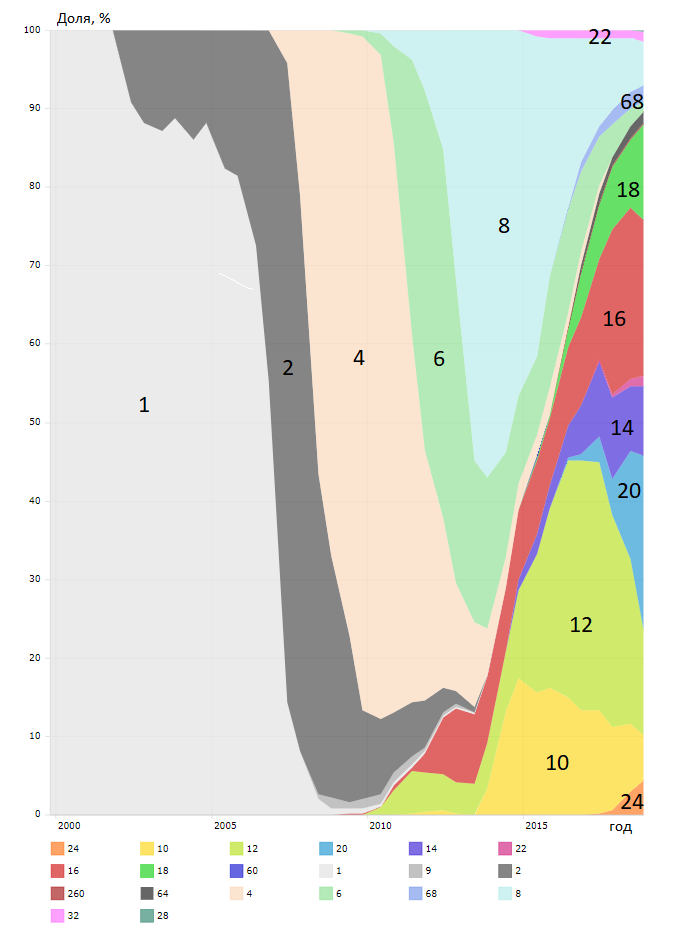
\includegraphics[width=1\linewidth]{graphPartOfMultiCoreProcessorFromYear}
		\caption{\textit{Частотность использования процессоров с различным числом ядер при создании суперкомпьютеров}}
		\label{graphPartOfMultiCoreProcessorFromYear:image}
	\end{figure}
	\parКак видим, активное использование двухъядерных процессоров в суперкомпьютерах началось уже в 2002 году, а примерно к 2005 году совершенно сошло на нет, тогда как в настольных компьютерах их применение в 2005 году лишь начиналось. На основании этого можно сделать простой прогноз распространённости многоядерных "настольных" процессоров к нужному году, если считать, что они в общих чертах повторяют развитие многоядерных архитектур суперкомпьютеров.
	\par
}
	{ %section1_2
	\subsection{Автоматическое распараллеливание программ}
	\Large\parПараллельное программирование – достаточно сложный ручной процесс, поэтому кажется очевидной необходимость его автоматизировать с помощью компилятора. Такие попытки делаются, однако эффективность автораспараллеливания пока что оставляет желать лучшего, т.к. хорошие показатели параллельного ускорения достигаются лишь для ограниченного набора простых for-циклов, в которых отсутствуют зависимости по данным между итерациями и при этом количество итераций не может измениться после начала цикла. Но даже если два указанных условия в некотором for-цикле выполняются, но он имеет сложную неочевидную структуру, то его распараллеливание производиться не будет. Виды автоматического распараллеливания:
	\begin{itemize}
		\item\textit{Полностью автоматический:}\quadучастие программиста не требуется, все действия выполняет компилятор.
		\item\textit{Полуавтоматический:}\quadпрограммист даёт указания компилятору в виде специальных ключей, которые позволяют регулировать некоторые аспекты распараллеливания.
	\end{itemize}
	\parСлабые стороны автоматического распараллеливания:
	\begin{itemize}
		\itemВозможно ошибочное изменение логики программы.
		\itemВозможно понижение скорости вместо повышения.
		\itemОтсутствие гибкости ручного распараллеливания.
		\itemЭффективно распараллеливаются только циклы.
		\itemНевозможность распараллелить программы со сложным алгоритмом работы.
	\end{itemize}
	\parПриведём примеры того, как с-программа в файле src.c может быть автоматически распараллелена при использовании некоторых популярных компиляторов:
	\begin{itemize}
		\itemКомпилятор GNU Compiler Collection:	 
gcc -O2 -floop-parallelize-all -ftree-parallelize-loops=K -fdump-tree-parloops-details src.c. При этом программисту даётся возможность выбрать значение параметра K, который рекомендуется устанавливать равным количеству ядер (процессоров). Особенностям реализации автораспараллеливания в gcc посвящён самостоятельный проект:\\ https://gcc.gnu.org/wiki/AutoParInGCC. 
		\itemКомпилятор фирмы Intel:	 
icc -c -parallel -par-report file.cc
		\itemКомпилятор фирмы Oracle:	 
solarisstudio -cc -O3 -xautopar -xloopinfo src.c
	\end{itemize}
}
	{ %section1_3
	\subsection{Основные подходы к распараллеливанию}
	\Large\parНа практике сложилось достаточное большое количество шаблонов параллельного программирования. Однако все эти шаблоны в своей основе используют всего два базовых подхода к распараллеливанию:
	\begin{itemize}
		\item\textbf{Распараллеливание по данным:} Программист находит в программе массив данных, элементы которого программа последовательно обрабатывает в некоторой функции func. Затем программист пытается разбить этот массив данных на блоки, которые могут быть обработаны в func независимо друг от друга. Затем программист запускает сразу несколько потоков, каждый из которых выполняет func, но при этом обрабатывает в этой функции отличные от других потоков блоки данных.
		\item\textbf{Распараллеливание по инструкциям :} Программист находит в программе последовательно вызываемые функции, процесс работы которых не влияет друг на друга (такие функции не изменяют общие глобальные переменные, а результаты одной не используются в работе другой). Затем эти функции программист запускает в параллельных потоках.
	\end{itemize}
	\parДва описанных метода легче понять на аналогии из обыденной жизни. Пусть два студента получили в стройотряде задание подмести улицу и покрасить забор. Если студенты решат использовать распараллеливание по данным, он будут сначала вместе подметать улицу, а затем вместе же красить забор. Если они решат использовать распараллеливание по инструкциям, то один студент полностью подметёт улицу, а другой покрасит в это время весь забор.
	\parВ большем числе случаев решение об использовании первого или второго метода является очевидным в силу внутренних особенностей распараллеливаемой программы. Однако некоторые задачи внешне одинаково хорошо распараллеливаются любым из двух методов. В этом случае выбор будет определяться тем, какой из методов более равномерно загружает потоки. В идеале все потоки должны приблизительно одновременно заканчивать выделенную им работу, чтобы оптимально загрузить ядра (процессоры) и чтобы закончившие работу потоки не простаивали в ожидании завершения работы соседними потоками.
	\par
}
	{ %section1_4
	\subsection{Методы синхронизации в параллельных программах}
	\parВ параллельных программах разработчик часто сталкивается с проблемой синхронизации между потоками. Как правило, проблемы возникают при доступе к памяти и одновременном выполнении каких-то критических участков кода - критических секций.
	\par\textbf{Критической областью} называют секцию программы, которая должна выполняться с исключительным правом доступа к разделяемым данным, на которые имеются ссылки в этой программе. Процесс, готовящийся войти в критическую область, может быть задержан, если любой другой процесс в это время выполняется в подобной критической области.
	\parВ этом разделе будут подробно рассмотрены механизмы синхронизации потоков на программном уровне.
	\parСуществуют следующие методы решения проблем синхронизации потоков:
		\begin{itemize}
			\item\textbf{Атомарные операции} - операции, которые выполняются целиком или не выполняются вовсе. Например, транзакция к БД является атомарной операцией. Когда два потока пытаются инкрементировать одну и ту же ячейку памяти несинхронизированно, значение может увеличиться на 2, а может и на 1 в зависимости от поведения потоков, так как операция инкрементации представляет собой как минимум 3 ассемблерные инструкции. Чтобы избежать этого стоит объявлять тип данных атомарным (если таковой есть в данном языке программирования/библиотеке). Частным случаем атомарных операций являются read-modify-write, compare-and-swap, test-and-set, fetch-and-add. Подробнее проблема реализации атомарных операций будет поднята в разделе\\~\ref{atomic:section} \textit{Атомарность операций в многопоточной программе}.
			\item\textbf{Семафор} - объект, ограничивающий число потоков, которые могут войти в эту область кода. Как правило это число задается при инициализации семафора. Затем при захвате семафора потоком проверяется количество потоков, захвативших семафор. Если максимальное количество потоков достигнуто, то поток будет ждать пока какой-то из потоков, вошедших в область кода, освободит его. Часто использование семафоров неоправдано, так как накладные расзоды на создание и поддержку семафора большие. Также следует избегать ''утечки семафора'', ситуации при которой поток не выходит из семафора при окончании выполнения области кода если программист забыл освободить ресурс.
			\item\textbf{Reader/writer semaphore} предоставляет потокам права \textit{только} на чтение или запись, причем во время записи данных одним потоком остальные потоки не имеет доступа к ресурсу. Однако в таких семафорах может быть проблема \textit{ресурсного голодания (starvation)}, при котором пока потоки будут читать данные, другие потоки не смогут записать данные долгий промежуток времени или наоборот. Частным решением этой проблемы при равном приоритете потоков может быть поочередный доступ потоков в очереди к доступи и записи.
			\item\textbf{Мьютекс} - частный случай семафора, при котором данную область кода может захватывать только один поток. Часто используется при организации управления критическими секциями, так как ''легче'' классического семафора. Следует отметить, что в стандарте языка C++11 кроме стандартного мьютекса существуют разные его модификации:  \textit{recursive\textunderscore mutex} - мьютекс, допускающий повторные захваты участка кода этим же потоком, \textit{timed\textunderscore mutex} - мьютекс с таймером захвата и  \textit{recursive\textunderscore timed\textunderscore mutex}, совмещающий достоинства обеих версий.
			\item\textbf{Spinlock (циклическая блокировка)} - блокировка, при которой поток в цикле ожидает освобождения ресурса. Не всегда является оптимальным решением, так как ожидающий поток работает во время ожидания. Внутри секции кода необходимо избегать прерываний, чтобы избежать deadlock'a.
			\item\textbf{Seqlock (последовательная блокировка)} - механизм синхронизации, предназначенный для быстрой записи переменной несколькими потоками. В ядре Linux работает следующим образом: поток ждет, пока критическая секция освободится(spinlock); при входе в секцию инкрементируется счетчик, поток делает свою работу. При выходе из секции поток проверяет значение счетчика. Если значение счетчика не изменилось, значит в данный момент никто не записывал данные и поток завершает работу, иначе он считывает значение переменной заново.
			\item\textbf{Knuth–Bendix сompletion algorithm} - одним из решений проблем синхронизации является алгоритм Кнута-Бендикса из курса дискретной математики. С его помощью можно перейти от последовательной программы к каскадной. Однако не для всех программ этот лагоритм работает, иногда он может уйти в бесконечный цикл или завершиться с ошибкой.
			\item\textbf{Barier (барьер)} - участок кода, в котором синхронизируется состояние потоков. Например, если для функции в главном потоке требуется чтобы все дочерние потоки закончили свою работу, можно поставить барьер перед ней. Тогда она будет ждать завершения работы дочерних потоков, после чего все потоки продолжат свою работу. Пример реализации барьера может быть критическая секция, код которой разрешается выполняться только последнему потоку, запросившему выполнение. Остальные потоки должны ожидать его.
			\item\textbf{Неблокирующие алгоритмы.} Часто бывает полезно не использовать стандартные приемы блокировки, а сделать алгоритм неблокирующим. В таком случае программист должен самостоятельно гарантировать, что критические секции кода не будут выполняться одновременно и целостность разделяемой памяти. Также плюсом таких алгоритмов является безопасная обработка прерываний. Для реализации таких адгоритмов часто используются другие технологии синхронизации: read-modify-write, CAS (см. раздел~\ref{atomic:section}) и другие.
			\item\textbf{RCU (read-copy-update)} - алгоритм, позволяющий потокам эффективно считывать данные, оставляя обновление данных на конец работы алгоритма, гарантируя при этом релевантные данные. Только один поток может писать данные, но читать данные могут сразу несколько потоков. Достигается это путем атомарной подмены указателя (CAS). Старые версии данных хранятся для прошлых обращений, пока на них есть хотя бы один указатель.
		\end{itemize}
	\parНесмотря на большое количество методов синхронизации чаще всего надо исходить из решаемой задачи. Например, если мы хотим сделать общую целочисленную переменную для нескольких потоков, нет смысла создавать mutex или semaphore, более оптимально сделать переменную атомарной. Всегда надо учитывать накладные расходы на создание блокировок и время разработки.
}
	{ %section1_5
	\subsection{Автоматическое распараллеливание программ}
	\parПараллельное программирование – достаточно сложный ручной процесс, поэтому кажется очевидной необходимость его автоматизировать с помощью компилятора. Такие попытки делаются, однако эффективность автораспараллеливания пока что оставляет желать лучшего, т.к. хорошие показатели параллельного ускорения достигаются лишь для ограниченного набора простых for-циклов, в которых отсутствуют зависимости по данным между итерациями и при этом количество итераций не может измениться после начала цикла. Но даже если два указанных условия в некотором for-цикле выполняются, но он имеет сложную неочевидную структуру, то его распараллеливание производиться не будет. Виды автоматического распараллеливания:
	\begin{itemize}
		\item\textit{Полностью автоматический:}\quadучастие программиста не требуется, все действия выполняет компилятор.
		\item\textit{Полуавтоматический:}\quadпрограммист даёт указания компилятору в виде специальных ключей, которые позволяют регулировать некоторые аспекты распараллеливания.
	\end{itemize}
	\parСлабые стороны автоматического распараллеливания:
	\begin{itemize}
		\itemВозможно ошибочное изменение логики программы.
		\itemВозможно понижение скорости вместо повышения.
		\itemОтсутствие гибкости ручного распараллеливания.
		\itemЭффективно распараллеливаются только циклы.
		\itemНевозможность распараллелить программы со сложным алгоритмом работы.
	\end{itemize}
	\parПриведём примеры того, как с-программа в файле src.c может быть автоматически распараллелена при использовании некоторых популярных компиляторов:
	\begin{itemize}
		\itemКомпилятор GNU Compiler Collection:	 
gcc -O3 -floop-parallelize-all -ftree-parallelize-loops=K -fdump-tree-parloops-details src.c. При этом программисту даётся возможность выбрать значение параметра K, который рекомендуется устанавливать равным количеству ядер (процессоров). Особенностям реализации автораспараллеливания в gcc посвящён самостоятельный проект:\\ \url{https://gcc.gnu.org/wiki/AutoParInGCC}. 
		\itemКомпилятор фирмы Intel:	 
icc -c -parallel -par-report file.cc
		\itemКомпилятор фирмы Oracle:	 
solarisstudio -cc -O3 -xautopar -xloopinfo src.c
	\end{itemize}
}
	{ %section1_6
	\subsection{Основные подходы к распараллеливанию}
	\parНа практике сложилось достаточное большое количество шаблонов параллельного программирования. Однако все эти шаблоны в своей основе используют три базовых подхода к распараллеливанию:
	\begin{itemize}
		\item\textbf{Распараллеливание по данным:} Программист находит в программе массив данных, элементы которого программа последовательно обрабатывает в некоторой функции func. Затем программист пытается разбить этот массив данных на блоки, которые могут быть обработаны в func независимо друг от друга. Затем программист запускает сразу несколько потоков, каждый из которых выполняет func, но при этом обрабатывает в этой функции отличные от других потоков блоки данных.
		\item\textbf{Распараллеливание по инструкциям:} Программист находит в программе последовательно вызываемые функции, процесс работы которых не влияет друг на друга (такие функции не изменяют общие глобальные переменные, а результаты одной не используются в работе другой). Затем эти функции программист запускает в параллельных потоках.
		\item\textbf{Распараллеливание по информационным потокам:} Программа представляет собой набор выполняемых функций, причем несколько функций могут ожидать результата выполнения предыдущих. В таком случае каждое ядро выполняет ту функцию, данные для которой уже готовы. Рассмотрим этот метод на примере абстрактного двухъядерного процессора, как наиболее сложный для понимания. Структурный алгоритм, изображенный на рисунке~\ref{structAlgorithm:image} состоит из 9 функций, некоторые из которых используют результат предыдущей функции в своей работе. Будем считать, что функция 3 использует результат работы функции 1, а функция 7 - результат функций 4 и 6 и тд, а также функция 5 выполняется по времени примерно столько же сколько функции 7, 8 и 9, вместе взятые. Тогда, на двухъядерной машине этот способ распараллеливания будет оптимальным решением.
	\end{itemize}
	\begin{figure}[H]
		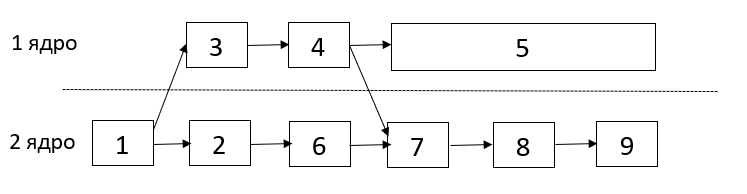
\includegraphics[width=1\linewidth]{structAlgorithm}
		\caption{\textit{Пример работы структурного алгоритма на двухъядерном процессоре}}
		\label{structAlgorithm:image}
	\end{figure}
	\parТри описанных метода легче понять на аналогии из обыденной жизни. Пусть два студента получили в стройотряде задание подмести улицу и покрасить забор. Если студенты решат использовать распараллеливание по данным, он будут сначала вместе подметать улицу, а затем вместе же красить забор. Если они решат использовать распараллеливание по инструкциям, то один студент полностью подметёт улицу, а другой покрасит в это время весь забор. Распараллелить по информационным потокам эту ситуацию не получится, так как эти два действия никак не зависят друг от друга. Если предположить, что им обоим нужны инструменты для работы, то один из них должен сначала сходить за ними, а потом она оба начнут делать свою работу.
	\parВ большем числе случаев решение об использовании метода является очевидным в силу внутренних особенностей распараллеливаемой программы. Выбор метода определяется тем, какой из них более равномерно загружает потоки. В идеале все потоки должны приблизительно одновременно заканчивать выделенную им работу, чтобы оптимально загрузить ядра (процессоры) и чтобы закончившие работу потоки не простаивали в ожидании завершения работы соседними потоками.
	\par
}
	{ %section1_7
	\subsection{Атомарность операций в многопоточной программе}
	\parОсновной проблемой при параллельном программировании является необходимость устранять конфликты при одновременном доступе к общей памяти нескольких потоков. Для решения этой проблемы обычно пытаются упорядочить доступ потоков к общим данным с помощью специальных средств – примитивов синхронизации. Однако возникает вопрос, существуют ли такие элементарные атомарные операции, выполнение которых несколькими потоками одновременно не требует синхронизации действий, т.к. эти операции выполнялись бы процессором "одним махом", или – как принято говорить – "атомарно" (т.е. никакая другая операция не может вытеснить из процессора предыдущую атомарную операцию до её окончания).
	\parТакими операциями являются практически все ассемблерные инструкции, т.к. они на низком уровне используют только те операции, которые присутствуют в системе команд процессора, а значит могут выполняться атомарно (непрерываемо). Однако при компиляции С программы команды языка С транслируются обычно в несколько ассемблерных инструкций. В связи с этим возникает вопрос о возможном существовании С-команд, которые компилируются в одну ассемблерную инструкцию. Такие команды можно было бы не "защищать" примитивами синхронизации (мьютексами) при параллельном программировании.
	\parОднако оказывается, что таких операций крайне мало, а некоторые из них могут вести себя как атомарно, так и не атомарно в зависимости от аппаратной платформы, для которой компилируется С-программа. Рассмотрим простейшую команду инкремента целочисленной переменной (тип int) в языке С: "w++". Можно легко убедиться (например, используя ключ "-S" компилятора gcc), что эта команда будет транслирована в три ассемблерные инструкции (взять из памяти, увеличить, положить обратно):
	\begin{figure}[H]
		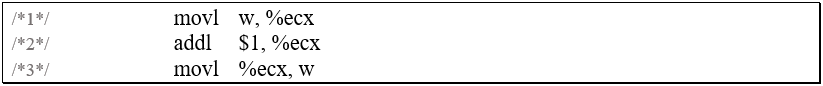
\includegraphics[width=1\linewidth]{AtomOperationExample1}
	\end{figure}
	\parЗначит, выполнять операцию инкремента некоторой переменной в нескольких потоках одновременно - небезопасно, т.к. при выполнении ассемблерной инструкции /*2*/ поток может быть прерван и процессор передан во владение другому потоку, который получит некорректное значение недоинкрементированной переменной.
	\parЛогично было бы предположить, что операции присваивания не должны обладать описанным недостатком. Действительно, в Ассемблере есть отдельная инструкция для записи значения переменной по указанному адресу. К сожалению, это предположение не до конца верно: действительно, при выполнении присваивания переменной типа char эта операция будет выполнена единой ассемблерной инструкцией. Однако с другими типами данных этого нельзя сказать наверняка. Общее практическое правило можно грубо сформулировать так: "атомарность операции присваивания гарантируется только для операций с данными, разрядность которых не превышает разрядности процессора". 
	\parНапример, при присваивании переменной типа int на 32-разрядном процессоре будет сгенерирована одна ассемблерная инструкция. Однако при компиляции этой же операции на 16-разрадном компьютере будет сгенерировано две ассемблерные команды для независимой записи младших и старших бит.
	\parСледует иметь в виду, что сформулированное правило работает при присваивании переменных и выражений, однако не всегда может выполняться при присваивании констант. Рассмотрим пример С-кода, в котором 64-разрядной переменной s (тип uint64\textunderscore t) присваивается большое число, заведомо превышающее 32-разрядную величину:
	\begin{figure}[H]
		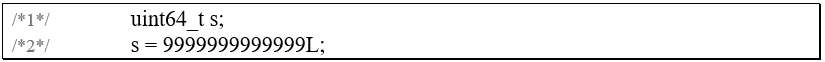
\includegraphics[width=1\linewidth]{AtomOperationExample2}
	\end{figure}
	\parЭтот код будет транслирован в следующий ассемблерный код на 64-разрядном процессоре:
	\begin{figure}[H]
		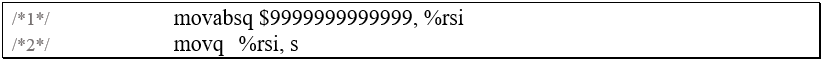
\includegraphics[width=1\linewidth]{AtomOperationExample3}
	\end{figure}
	\parКак видим, операция присваивания была транслирована в две ассемблерные инструкции, что делает невозможным безопасное распараллеливание такой операции.
	\parСформулированное правило применимо не только к операции присваивания, но и к операции чтения переменной из памяти, поэтому любую из этих операций в потокобезопасной среде придётся защищать мьютексами или критическими секциями.
	\parОсобый случай атомарного изменения данных - это изменение структуры. Для этого надо использовать CAS-операцию с указателем на эту структуру. Выполняя такую операцию, процессор создаст вторую структуру данных с заданными полями и сравнит её со старой версией структуры. Если значение хотя бы одного поля поменялось, то он атомарно подменит указатель. В этом есть накладные расходы: даже простое изменение одного поля структуры требует создание полной копии структуры, чтобы потом подменить указатель.
	\par
}
}
	{ %section2
	\section{Показатели эффективности параллельной программы}
	{ %section2_1
	\subsection{Параллельное ускорение и параллельная эффективность}
	\parДля оценки эффективности параллельной программы принято сравнивать показатели скорости исполнения этой программы при её запуске на нескольких идентичных вычислительных системах, которые различаются только количеством центральных процессоров (или ядер). На практике, однако, редко используют для этой цели несколько независимых аппаратных платформ, т.к. обеспечить их полную идентичность по всем параметрам достаточно сложно. Вместо этого, измерения проводятся на одной многопроцессорной (многоядерной) вычислительной системе, в которой искусственно ограничивается количество процессоров (ядер), задействованных в вычислениях. Это обычно достигается одним из следующих способов:
	\begin{itemize}
		\itemУстановка аффинности процессоров (ядер).
		\itemВиртуализация процессоров (ядер).
		\itemУправление количеством нитей.
	\end{itemize}
	\textbf{Установка аффинности.} Под аффинностью (processor affinity/pinning) понимается указание операционной системе запускать указанный поток/про-\\цесс на явно заданном процессоре (ядре). Установить аффинность можно либо с помощью специального системного вызова изнутри самой параллельной программы, либо некоторым образом извне параллельной программы (например, средствами ''Диспетчера задач'' или с помощью команды ''start'' с ключом ''/AFFINITY'' в ОС MS Windows, или команды ''taskset'' в ОС Linux). Недостатки этого метода:
	\begin{itemize}
		\itemНеобходимость модифицировать исследуемую параллельную программу (при использовании системного вызова изнутри самой программы).
		\itemНевозможность управлять аффиностью на уровне потоков, т.к. обычно ОС позволяет устанавливать аффинность только для процессов (при установке аффиности внешними по отношению к параллельной программе средствами).
	\end{itemize}
	\textbf{Виртуализация процессоров (ядер).} При создании виртуальной ЭВМ в большинстве специализированных программ (например, VMWare, \\VirtualBox) есть возможность "выделить" создаваемой виртуальной машине не все присутствующие в хост-системе процессоры (ядра), а только часть из них. Это можно использовать для имитации тестового окружения с заданным количеством ядер (процессоров). Например, на рисунке~\ref{VirtualBoxNumberCores:image} показано, что для настраиваемой виртуальной машины из восьми доступных физических (и логических) процессоров доступными являются только три.
	\begin{figure}[H]
		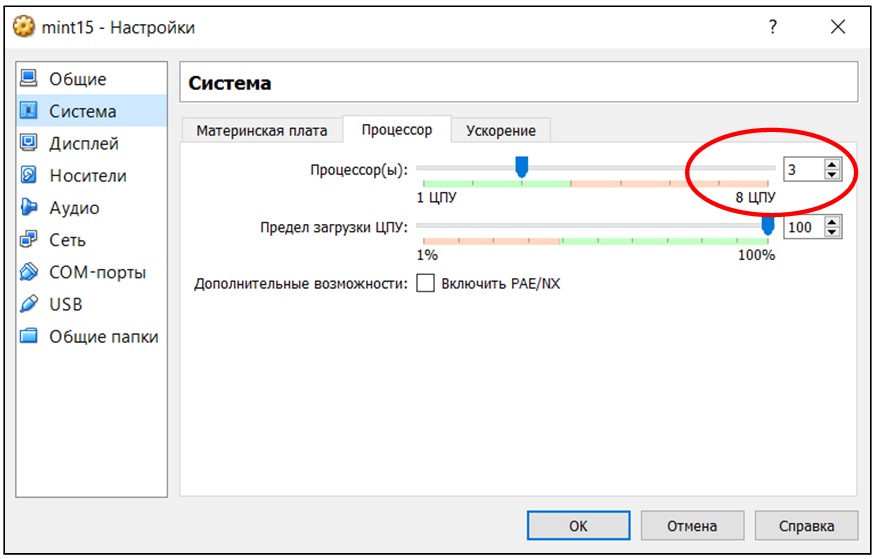
\includegraphics[width=1\linewidth]{VirtualBoxNumberCores}
		\caption{\textit{Выбор количества виртуальных процессоров в Oracle VirtualBox}}
		\label{VirtualBoxNumberCores:image}
	\end{figure}
	\parНедостатком описанного подхода являются накладные расходы виртуализации, которые непредсказуемым образом могут сказаться на результатах экспериментального измерения производительности параллельной программы. Достоинством виртуализации (по сравнению с управляемой аффинностью) является более естественное поведение тестируемой программы при использовании доступных процессоров, т.к. ОС не даётся жёстких указаний, что те или иные потоки всегда должны быть "привязаны" к заранее заданным процессорам (ядрам) – эта особенность позволяет более точно воспроизвести сценарий потенциального "живого" использования тестируемой программы, что повышает достоверность получаемых замеров производительности. 
	\par\textbf{Управление количеством нитей.} При создании параллельных программ достаточно часто количество создаваемых в процессе работы программы нитей не задаётся в виде жёстко фиксированной величины. Напротив, оно является гибко конфигурируемой величиной p, выбор значения которой позволяет оптимальным образом использовать вычислительные ресурсы той аппаратной платформы, на которой запускается программа. Это позволяет программе "адаптироваться" под то количество процессоров (ядер), которое есть в наличии на конкретной ЭВМ.
	\parЭту особенность параллельной программы можно использовать для экспериментального измерения её показателей эффективности, для чего параллельную программу запускают при значениях $p = 1,2,…,n$, где $n$ – это количество доступных процессоров (ядер) на используемой для тестирования многопроцессорной аппаратной платформе. Описанный подход позволяет искусственно ограничить количество используемых при работе программы процессоров (ядер), т.к. в любой момент времени параллельная программа может исполняться не более, чем на $p$ вычислителях. Анализируя измерения скорости работы программы, полученные для различных $p$, можно рассчитать значения некоторых показателей эффективности распараллеливания (см. ниже).
	\par\textbf{Параллельное ускорение (parallel speedup).} В отличие от применяемого в физике понятия величины ускорения как прироста скорости в единицу времени, в программировании под параллельным ускорением понимают безразмерную величину, отражающую прирост скорости выполнения параллельной программы на заданном количестве процессоров по сравнению с однопроцессорной системой, т.е.
	\begin{equation}
		\label{parallelAcceleration:equation}
		S(p)\;=\;\frac{V(p)}{V(1)},
	\end{equation}
	где V(p) – средняя скорость выполнения программы на $p$ процессорах (ядрах), выраженная в условных единицах работы в секунду (УЕР/с). Примерами УЕР могут быть количество просуммированных элементов матрицы, количество обработанных фильтром точек изображения, количество записанных в файл байт и т.п.
	\parСчитается, что значение $S(p)$ никогда не может превысить $p$, что на интуитивном уровне звучит правдоподобно, ведь при увеличении количества работников, например, в четыре раза невозмножно добиться выполнения работы в пять раз быстрее.  Однако, как мы рассмотрим ниже, в экспериментах вполне может наблюдаться сверх-линейное параллельное ускорение при увеличении количества процессоров. Конечно, такой результат чаще всего означает ошибку экспериментатора, однако существуют ситуации, когда этот результат можно объяснить тем, что при увеличении количества процессоров не только кратно увеличивается их вычислительный ресурс, но так же кратно увеличивается объём кэш-памяти первого уровня, что позволяет в некоторых задачах существенно повысить процент кэш-попаданий и, как следствие, сократить время решения задачи.
	\par\textbf{Параллельная эффективность (parallel efficiency).} Хотя величина параллельного ускорения является безразмерной, её анализ не всегда возможен без информации о значении $p$. Например, пусть в некотором эксперименте оказалось, что $S(p)=10$. Не зная значение $p$, мы лишь можешь сказать, что при параллельном выполнение программа стала работать в 10 раз быстрее. Однако если при этом $p=1000$, это ускорение нельзя считать хорошим достижением, т.к. в других условиях можно было добиться почти 1000 кратного прироста скорости работы и не тратить столь внушительные ресурсы на плохо распараллеливаемую задачу. Напротив, при значении $p=11$ можно было бы счесть  величину $S(p)=10$ вполне приемлемой.
	\parЭта проблема привела к необходимости определить ещё один показатель эффективности параллельной программы, который бы позволил получить некоторую оценку эффективности распараллеливания с учётом  количества процессоров (ядер). Этой величиной является \textbf{параллельная эффективность}
	\begin{equation}
		\label{parallelEffect:equation}
		E(p)\;=\;\frac{S(p)}p\;=\;\frac{V(p)}{p\cdot\;V(1)}
	\end{equation}
	\parСреднюю скорость выполнения программы $V(p)$ можно измерить следующими двумя \textit{неэквивалентными} методами:
	\begin{itemize}
		\item\textbf{Метод Амдала:} рассчитать $V(p)$, зафиксировав объём выполняемой работы (при этом изменяется время выполнения программы для различных $p$).
		\item\textbf{Метод Густавсона-Барсиса:} рассчитать $V(p)$, зафиксировав время работы тестовой программы (при этом изменяется количество выполненной работы для различных $p$).
	\end{itemize}
	Рассмотрим подробнее каждый из указанных методов в двух следующих подразделах.
	\par
}
	{ %section2_2
	\subsection{Метод Амдала}
	\parПри оценке эффективности распараллеливания некоторой программы, выполняющей фиксированный объём работы, скорость выполнения можно выразить следующим образом:$\left.V(p)\right|_{w=const}\;=\;\frac w{t(p)}$, где $w$ – это общее количество УЕР, содержащихся в рассматриваемой программе, $t(p)$ – время выполнения работы w при использовании $p$ процессоров. Тогда выражение для параллельного ускорения примет вид:
	\begin{equation}
		\label{AmdalSFromP:equation}
		\left.S(p)\right|_{w=const}\;=\;\frac{V(p)}{V(1)}\;=\;\frac w{t(p)}\;=\;\frac w{t(1)}\;=\;\frac{t(1)}{t(p)}.
	\end{equation}
	\parЗапишем время $t(1)$ следующим образом:
	\begin{equation}
		t(1)\;=\;t(1)\;+\;(k\;\cdot\;t(1)\;-\;k\;\cdot\;t(1))\;=\;k\;\cdot\;t(1)\;+\;(1\;-\;k)\;\cdot\;t(1),
	\end{equation}
	где $k\;\in\;\lbrack0,1)$ - это коэффициент распараллеленности программы, которым мы обозначим долю времени, в течение которого выполняется идеально распараллеленный код внутри рассматриваемой программы. Такой код можно выполнить ровно в $p$ раз быстрее, если количество процессоров увеличить в p раз. Заметим, что коэффициент $k$ никогда не равен единице, т.к. в любой программе всегда присутствует нераспараллеливаемый код, который приходится выполнять последовательно на одном процессоре (ядре), даже если их доступно несколько. Если для некоторой программы $k=0$, то при запуске этой программы на любом количестве процессоров $p$ она будет решаться за одинаковое время.
	\parУчитывая, что в методе Амдала количество работы остаётся неизменным при любом $p$ (т.к. $w=const$), можно утверждать, что значение $k$ не изменяется в проводимых экспериментах, следовательно можем записать:
	\begin{equation}
		\label{AmdalTFromP:equation}
		t(p)\;=\;\frac{k\;\cdot\;t(1)}p\;+\;(1\;-\;k)\;\cdot\;t(1),
	\end{equation}
	где первое слагаемое даёт время работы распараллеленного в p раз идеально распараллеливаемого кода, а второе слагаемое – время работы нераспараллеленного кода, которое не меняется при любом $p$. Подставив формулу~\eqref{AmdalTFromP:equation} в~\eqref{AmdalSFromP:equation}, получим выражение $$\left.S(p)\right|_{w=const}\;=\;\frac{t(1)}{t(p)}\;=\;\frac{t(1)}{{\displaystyle\frac{k\;\cdot\;t(1)}p}\;+\;(1\;-\;k)\;\cdot\;t(1)}\;=\;\frac1{{\displaystyle\frac kp}\;+\;1\;-\;k},$$ которое перепишем в виде
	\begin{equation}
		\label{AmdalLaw:equation}
		\left.S(p)\right|_{w=const}\;=\;S_A(p)\;=\;\left(\frac kp\;+\;1\;-\;k\right)^{-1}
	\end{equation}
	более известном как \textbf{закон Амдала} – по имени американского учёного Джина Амдала, предложившего это выражение в 1967 году. До сих пор в специализированной литературе по параллельным вычислениям именно этот закон является основополагающим, т.к. позволяет получить теоретическое ограничение сверху для скорости выполнения некоторой заданной программы при распараллеливании.
	\parГрафик зависимости параллельного ускорения от количества ядер изображен на рисунке~\ref{GraphAmdalSFromP:image}:
	\begin{figure}[H]
		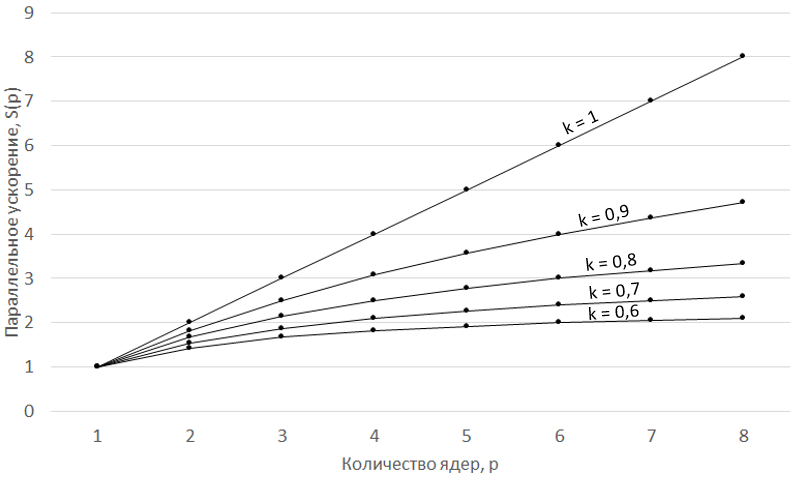
\includegraphics[width=1\linewidth]{GraphAmdalSFromP}
		\caption{\textit{График зависимости параллельного ускорения от количества ядер по Амдалу}}
		\label{GraphAmdalSFromP:image}
	\end{figure}
	\parОтметим, что выражение для расчёта параллельной эффективности при использовании метода Амдала можно получить, объединив формулы~\eqref{parallelEffect:equation} и~\eqref{AmdalLaw:equation}, а именно:
	\begin{equation}
		E_A(p)\;=\;\left(k\;+\;p\;-\;p\;\cdot\;k\right)^{-1}
	\end{equation}
	\parВажным допущением закона Амдала является идеализация физического смысла величины $k$, состоящая в предположении, что идеально распараллеленный код будет давать линейный прирост скорости работы при изменении $p$ от $0$ до $+\infty$ . При решении реальных задач приходится ограничивать этот интервал сверху некоторым конечным положительным значением $p_{max}$ и/или исключать из этого интервала все значения, не кратные некоторой величине, обычно задающей размерность задачи.
	\parНапример, код программы, выполняющей конволюционное кодирование независимо для пяти равноразмерных файлов, может давать линейное ускорение при изменении $p$ от $1$ до $5$, но уже при $p=6$ скорее всего покажет нулевой прирост скорости выполнения задачи (по сравнению с решением при $p=5$). Это объясняется тем, что  конволюционное кодирование, также известно как ''свёрточное'', является принципиально нераспараллеливаемым при кодировании выбранного блока данных.
	\par
}
	{ %section2_3
	\subsection{Метод Густавсона-Барсиса}
	\parПри оценке эффективности распараллеливания некоторой программы, работающей фиксированное время, скорость выполнения можно выразить следующим образом: $\left.V(p)\right|_{t=const}\;=\;\frac {w(p)}t$, где $w(p)$ – это общее количество УЕР, которые программа успевает выполнить за время $t$ при использовании $p$ процессоров. Тогда выражение~\eqref{parallelAcceleration:equation} для параллельного ускорения примет вид:
	\begin{equation}
		\label{GustavsonAcceleration:equation}
		\left.S(p)\right|_{t=const}\;=\;\frac{V(p)}{V(1)}\;=\;\frac{w(p)}t\;:\;\frac{w(1)}t\;=\;\frac{w(p)}{w(1)}.
	\end{equation}
	\parЗапишем количество работы $w(1)$ следующим образом:
	\begin{equation}
		\label{GustavsonWork:equation}
		w(1)\;=\;w(1)\;+\;(k\;\cdot\;w(1)\;-\;k\;\cdot\;w(1))\;=\;k\;\cdot\;w(1)\;+\;(1\;-\;k)\;\cdot\;w(1),
	\end{equation}
	где $k\in\lbrack0,1)$ – это уже упомянутый ранее коэффициент распараллеленности программы. Тогда первое слагаемое можно считать количеством работы, которая идеально распараллеливается, а второе – количество работы, которую распараллелить не удается при добавлении процессоров (ядер).
	\parПри использовании $p$ процессоров количество выполненной работы $w(p)$ очевидно станет больше, при этом оно  будет состоять из двух слагаемых: 
	\begin{itemize}
		\itemколичество нераспараллеленных условных единиц работы $(1-k)\cdot w(1)$, которое не изменится по сравнению с формулой~\eqref{GustavsonWork:equation}.
		\itemколичество распараллеленных УЕР, объём которых увеличиться в $p$ раз по сравнению с формулой~\eqref{GustavnsonWork:equation}, т.к. в работе будет задействовано $p$ процессоров вместо одного.
	\end{itemize}
	\parУчитывая сказанное, получим следующее выражение для $w(p)$:
	\par$w(p)\;=\;p\;\cdot\;k\;\cdot\;w(1)\;+\;(1\;-\;k)\;\cdot\;w(1),$ тогда с учетом формулы~\eqref{GustavsonAcceleration:equation} получим: $\;\frac{w(p)}{w(1)}=\;\frac{p\cdot k\cdot w(1)+(1-k)\cdot w(1)}{w(1)}$, что позволяет записать:
	\begin{equation}
		\left.S(p)\right|_{t=const}\;=\;S_{GB}(p)\;=\;p\;\cdot\;k\;+\;1\;-\;k
	\end{equation}
	\parПриведённое выражение называется \textbf{законом Густавсона-Барсиса}, который Джон Густавсон и Эдвин Барсис сформулировали в 1988 году. 
	\par
}
	{ %section2_4
	\subsection{Модификация закона Амдала (по проф. Бухановскому)}
	\parВ реальных вычислительных системах ОС тратит ресурсы на создание и удаление новых потоков. Время, затраченное на эти операции не учитывается в законе Амдала. Параллельное ускорение $S(p)$ зависит от количества ядер и доли распараллеливаемых операций, но не зависит от количества последних. Выведем формулу в которой количество операций для которых необходимо создать поток будет учитываться.
	\parПусть $N$ – количество распараллеливаемых операций, $M$ – количество нераспараллеливаемых операций, $t_c$ – время выполнения одной операции, $p$ – количество вычислителей(ядер), $T_i$ – время выполнения программы при использовании $i$ параллельных потоков на $i$ вычислителях, $\alpha$ – некий масштабирующий коэффициент, инкапсулирующий в себе количество времени, требуемого на создание, удаление потока и прочие накладные операции. 
По формуле~\eqref{AmdalSFromP:equation}, $S(p)\;=\;\frac{T_1}{T_p}$.
	\parНайдем сначала $T_1$. Так как это код выполняется линейно, то время затраченное на его выполнение будет равно количеству операций помноженному на время выполнения одной операции: $T_1\;=\;t_c(N\;+\;M)$. 
	\parВремя выполнение распараллельнной программы $T_p$ включается в себя время на создание потока: $t_c\alpha(p\;-\;1)N$ (нужно создать $(p\;-\;1)$ новых потоков, так как главный поток уже создан и для каждого затратить какое-то время $\alpha$), время работы распараллеливаемоего кода на всех ядрах: $\frac {t_cN}p$ и время работы нераспараллеливаемого кода $t_cM$. Итого, разделив $T_1$ на $T_p$, получим формулу закона Амдала по проф. Бухановскому:
	\begin{equation}
		\label{AmdalBuhunovsky:equation}
		S(p,N)\;=\;\frac{T_1}{T_p}\;=\;\frac{N\;+\;M}{\alpha(p\;-\;1)N\;+\;\frac Np\;+\;M}
	\end{equation}
	Из формулы~\eqref{AmdalBuhunovsky:equation} видно, что с ростом количество ядер после определенного предела $S(p,N)$  не будет расти как в законе Амдала, так как время будет тратиться много времени на создание новых потоков. На рисунке~\ref{GraphAmdalBuhunovsky:image} наглядно видно, что $S(p,N)$ уменьшается при большом количестве потоков и становится заметно меньше $S(p)$ по Амдалу даже при небольшом значении $\alpha$.
	\begin{figure}[H]
		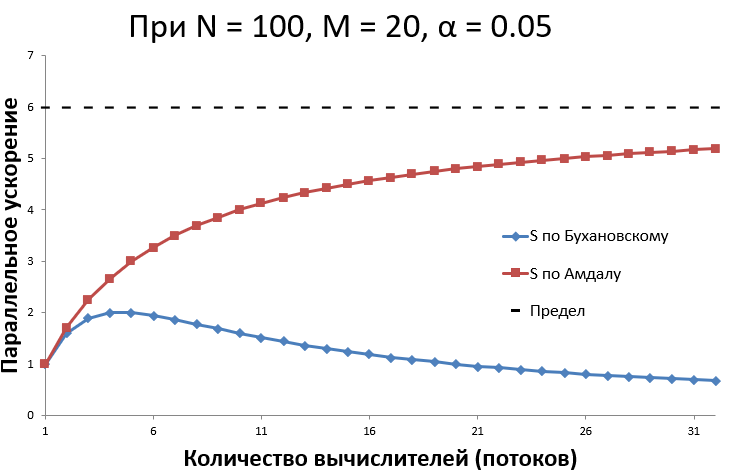
\includegraphics[width=1\linewidth]{GraphAmdalBuhunovsky}
		\caption{\textit{График зависимости параллельного ускорения от количества потоков}}
		\label{GraphAmdalBuhunovsky:image}
	\end{figure}
}
	{ %section2_5
	\subsection{Измерение времени выполнения параллельных программ}
	\par\textbf{Инструменты измерения времени.} Измерение времени работы программы в языке С не является сложной проблемой, однако при параллельном программировании возникает ряд специфических сложностей при выполнении этой операции. Далеко не все функции, пригодные для измерения времени работы последовательной программы, подойдут для измерения времени работы многопоточной программы. 
	\parНапример, если в однопоточной программе для измерения времени работы участка кода использовать функции ctime или localtime, то они успешно справятся с поставленной задачей. Однако после распараллеливания этого участка кода возможно возникновение трудноидентифицируемых проблем с неправильным измерением времени, т.к. обе указанные функции имеют внутреннюю static-переменную, которая при попытке изменить её одновременно несколькими потоками может принять непредсказуемое значение.
	\parС целью решить описанную проблему в некоторых C-компиляторах (например, gcc) были реализованы потокобезопасные (thread-safe, re-entrant) версии этих функций: ctime\textunderscore r и localtime\textunderscore r. К сожалению, эти функции доступны не во всех компиляторах. Например, в компиляторе Visual Studio аналогичную проблему решили использованием функций с совсем иными именами и API: GetTickCount, GetLocalTime, GetSystemTime. Перечислим для полноты изложения некоторые другие gcc-функции, которые также позволяют измерять время: time, getrusage, gmtime, gettimeofday.
	\parЕщё одна стандартная С-функция clock также не может быть использована для измерения времени выполнения многопоточных программ. Однако причина этого не в отсутствии реэнтерабельности, а в особенностях способа, которым эта функция рассчитывает прошедшее время: clock возвращает количество тиков процессора, которые были выполнены при работе программы суммарно всеми её потоками. Очевидно, что это количество остается почти неизменным при выполнении программы разным количеством потоков (''почти'', т.к. накладные расходы на создание, удаление и управление потоками предлагается в целях упрощения изложения считать несущественными).
	\parВ итоге оказалось, что удовлетворительного \textit{кросс-платформенного} решения для потокобезопасного измерения времени с высокой точностью (до микросекунд) средствами чистого языка С пока не существует. Проблему, однако, можно решить, используя сторонние библиотеки, выбирая те из них, которые имеют реализацию на целевых платформах. 
	\parВыгодно выделяется среди таких библиотек система OpenMP, которая реализована в абсолютном большинстве современных компиляторов для всех современных операционных систем. В OpenMP есть две функции для измерения времени: omp\textunderscore get\textunderscore wtime и omp\textunderscore get\textunderscore wtick, которые можно использовать в С-программах, если подключить заголовочный файл omp.h и при компиляции указать нужный ключ (например, в gcc это ключ ''-fopenmp'').
	\par\textbf{Погрешность измерения времени.} Другим интересным моментом при измерении времени работы параллельной программы является способ, с помощью которого исследователь исключает из замеров различные случайные погрешности, неизбежно возникающие при эксперименте в работающей операционной системе, которая может начать процесс обновления или оптимизации, не уведомляя пользователя. Общепринятыми является способ, при котором исследователь проводит не один, а сразу N экспериментов с параллельной программой, не меняя исходные данные. Получается N замеров времени, которые в общем случае будут различными вследствие различных случайных факторов, влияющих на проводимый эксперимент. Далее чаще всего используется один из следующих методов:
	\begin{enumerate}
		\item\textit{Расчёт доверительного интервала:} с учётом всех N измерений рассчитывается доверительный интервал, например, с помощью метода Стьюдента.
		\item\textit{Поиск минимального замера:} среди N измерений выбирается наименьшее и именно оно используется в качестве окончательного результата.
	\end{enumerate}
	\parПервый метод даёт корректный результат, только если ошибки замеров распределены по нормальному закону. Чаще всего это так, поэтому применение метода оправдано и к позволяет получить дополнительную информацию о возможном применении тестируемой программы в живых условиях работающей ОС.
	\parВторой метод не предъявляет требований к виду закона распределения ошибки измерений и этим выгодно отличается от предыдущего. Кроме того, при больших N выбор минимального замера позволит с большой вероятностью исключить из эксперимента все фоновые влияния операционной системы и получить в качестве результата точное измерение времени работы программы в идеальных условиях. 
	\par\textbf{Практический пример.} Сравним на примере описанные выше методы избавления от погрешности экспериментальных замеров времени. Будем измерять накладные расходы OpenMP на создание и удаление потоков следующим образом:
	\begin{figure}[H]
		\lstinputlisting{OpenMPExampleTimeMeasurement.cpp}
	\end{figure}
	В строке 2 мы даём OpenMP указание, чтобы при входе в параллельную область, расположенную далее в программе, было создано i потоков. Если не давать этого указания, OpenMP создаст количество потоков по количеству доступных в системе вычислителей (ядер или логических процессоров). В строке 4 мы запускаем параллельную область программы, OpenMP создаёт i потоков. В строке 5 мы даём указание выполнять последующую простейшую инструкцию лишь в одном потоке (остальные потоки не будут делать никакой работы. Это нужно, чтобы в замеряемое время работы попали только расходы на создание/удаление потоков, а все прочие расходы терялись бы на их фоне. В строке 6 заканчивается параллельная область, OpenMP удаляет из памяти i потоков. Более подробное описание использованных команд OpenMP можно найти в разделе~\ref{OpenMP:section} \textit{''Технология OpenMP''} данного учебного  пособия.
	\parЭксперименты с приведённой программой проводились на компьютере с процессором Intel Core i5 (4 логических процессора) с 8 гигабайт ОЗУ в операционной системе Debian Wheezy. Опытным путём было выявлено, что использованная операционная система на доступной аппаратной платформе не может создать более 381 потока в OpenMP-программе (этим объясняется значение в строке 1). Было проведено в общей сложности N=100 экспериментов, результаты которых обрабатывались каждым из двух описанных методов. Полученные результаты приведены на рисунке~\ref{OpenMPExpensesOnCreatingThreads:image}.
	\begin{figure}[H]
		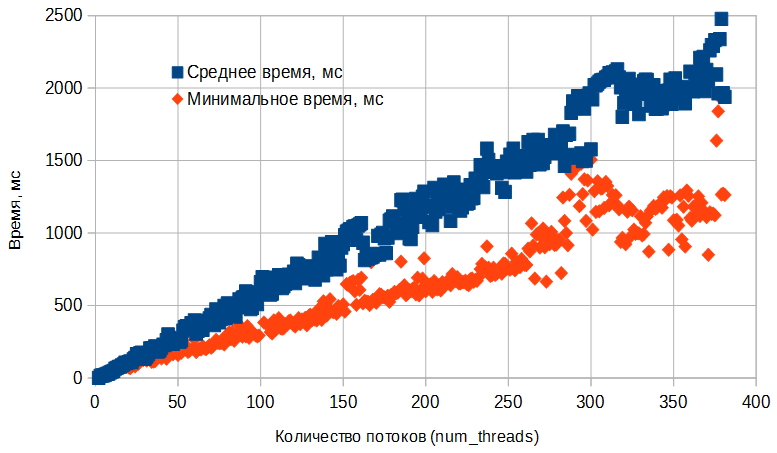
\includegraphics[width=1\linewidth]{OpenMPExpensesOnCreatingThreads}
		\caption{\textit{Результаты измерения накладных расходов OpenMP при создании и удалении потоков}}
		\label{OpenMPExpensesOnCreatingThreads:image}
	\end{figure} 
	\parПо оси ординат откладывается измеренная величина (T2 - T1) в миллисекундах, по оси абсцисс – значения переменной i, означающие количество создаваемых потоков. Верхний график, состоящий из синих квадратов, показывает усреднённую величину (T2 - T1) по 100 проведённым экспериментам. Доверительный интервал при этом не показан, т.к. он загромождал бы график, не добавляя информативности, однако ширина доверительного интервала с уровнем доверия 90\% приблизительно соответствует разбросу по вертикали квадратов верхнего графика для соседних значений i. 
	\parНижний график, состоящий из ромбов, представляет собой минимальные из 100 проведённых замеров величины (T2 -  T1) для указанных на оси абсцисс значений i. Видим, что даже большого количества экспериментов оказалось недостаточно, чтобы нижний график имел бы гладкую непрерывную структуру без заметных флуктуаций.

}
}
	{ %section3
	\section{Практические аспекты параллельного программирования}
	{ %section3_1
	\subsection{Отладка параллельных программ}
	\Large\parСредства отладки параллельных программ встроены в большинство популярных интегрированных сред разработки (IDE), например: Visual Studio, Eclipse CDT, Intel Parallel Studio и т.п. Эти средства включают в себя удобную визуализацию временных диаграмм исполнения потоков, автоматический поиск подозрительных участков программы, в которых могут наблюдаться гонки данных и взаимоблокировки.
	\parНесмотря на эффективность существующих инструментов отладки, при работе в дебаггере (debugger) с параллельной программой возникают существенные затруднения, т.к. для своего корректного функционирования отладчик добавляет в машинный код исходной параллельной программы дополнительные инструкции, которые изменяют временную диаграмму выполнения потоков по отношению друг к другу. Это может приводить к ситуациям, когда при тестировании программы в отладчике не наблюдаются гонки данных и взаимоблокировки, которые при запуске Release-версии программы проявятся в полной мере.
	\parТакже при отладке многопоточной программы следует иметь в виду, что её поведение (как при штатной работе, так и при отладке) может существенным образом различаться при использовании одноядерного и многоядерного процессора. При запуске нескольких потоков на одноядерной машине они будут выполняться в режиме разделения времени, т.е. последовательно. Значит, в этом случае не будут наблюдаться многие проблемы с совместным доступом к памяти и обеспечением когерентности кэшей, присущие многоядерным системам. Кроме того, при отладке программы на одноядерной системе программист может использовать неявные приёмы обеспечения последовательности выполнения операций. 
	\parНапример, программист может некорректно предполагать, что при выполнении высокоприоритетного потока низкоприоритетный поток не может завладеть процессором. Это предположение корректно только в одноядерной системе, ведь при наличии нескольких ядер и малом количестве высокоприоритетных потоков вполне может наблюдаться ситуация, когда низкоприоритетный поток завладеет одним из ядер, при одновременной работе высокоприоритетного потока на соседнем ядре.
	\par
}
	{ %section3_2
	\subsection{Менеджеры управления памятью для параллельных программ}
	\parПри вызове функций malloc/free в однопоточной программе не возникает проблем даже при довольно высокой интенсивности вызовов одной из них. Однако в параллельных программах эти функции могут стать узким местом, т.к. при их одновременном использовании из нескольких потоков происходит блокировка общего ресурса (менеджера управления памятью), что может привести к существенной деградации скорости работы многопоточной программы.
	\parПолучается, что несмотря на формальную потокобезопасность стандартных функций работы с памятью, они могут стать потоконеэффективными при очень интенсивной работе с памятью нескольких параллельно работающих потоков.
	\parДля решения этой проблемы существует ряд сторонних программ, называющихся "Менеджер управления памятью (МУП)" (Memory Allocator), как платных, так и бесплатных с открытым исходным кодом. Каждое из них обладает своими достоинствами и недостатками, которые следует учитывать при выборе. Перечислим наиболее распространённые МУП с указанием ссылок на официальные сайты:
	\begin{itemize}
		\sloppy
		\item tcmalloc: \url{http://goog-perftools.sourceforge.net/doc/tcmalloc.html}
		\item ptmalloc: \url{http://www.malloc.de/malloc/ptmalloc3-current.tar.gz}
		\item dmalloc: \url{http://dmalloc.com/}
		\item HOARD: \url{http://www.hoard.org/}
		\item nedmalloc: \url{http://www.nedprod.com/programs/portable/nedmalloc/}
	\end{itemize}
	\parПеречисленные МУП разработаны таким образом, что ими можно "незаметно" для параллельной программы подменить стандартные МУП библиотеки libc языка С. Это значит, что выбор конкретного МУП никак не влияет на исходный код программы, поэтому общая практика использования сторонних МУП такова: параллельная программа изначально создаётся с использованием МУП libc, затем проводится профилирование работающей программы, затем при обнаружении узкого места (bottleneck) в функциях malloc/free принимается решение заменить стандартный МУП одним из перечисленных.
	\parТакже стоит отметить, что некоторые технологии распараллеливания (например, Intel TBB) уже имеют в своём составе специализированный МУП, оптимизированный для выполнения в многопоточном режиме.
	\par
}
	{ %section3_3
	\subsection{Технология OpenMP}
	\Large\par\textbf{Краткая характеристика технологии.} Первая версия стандарта OpenMP появилась в 1997 году при поддержке крупнейших IT-компаний мира (Intel, IBM, AMD, HP, Nvidia и др.). Целью нового стандарта было предложить кроссплатформенный инструмент для распараллеливания, который был бы более высокоуровневый, чем API управления потоками, предлагаемые операционной системой. На данный момент OpenMP стандартизована для трёх языков программирования: С, С++ и Фортран.
	\par\textbf{Поддержка компиляторами.} Абсолютное большинство существующих современных компиляторов С/С++ поддерживают OpenMP версии 2.0 (например, как gcc, так и Visual Studio). Однако лишь немногие компиляторы поддерживают более новую версию OpenMP 4.0, поэтому далее при изложении материала будет в качестве "общего знаменателя"\verb+ +использоваться технология OpenMP 2.0.
	\par OpenMP определяет набор директив препроцессору, которые дают указание компилятору заменить следующий за ними исходный код на его параллельную версию с помощью доступных компилятору средств, например с помощью POSIX Threads в Linux или Windows Threads в операционных системах Microsoft. Для корректной трансляции директив необходимо при компиляции указать специальный ключ, значение которого зависит от компилятора (примеры приведены в таблице~\ref{compilerOpenMP:table}).
	\begin{table}[H]
		\Large
		\caption{Ключи компиляторов для запуска OpenMP}
		\label{compilerOpenMP:table}
		\begin{center}
			\begin{tabular}{|c|c|}
				\hline
				\textbf{Название компилятора} & \specialcell{\textbf{Ключ компилятору для включения} \\  \textbf{OpenMP}} \\
				\hline
				Gcc & -fopenmp \\
				\hline
				icc (Intel C/C++ compiler) & -openmp \\
				\hline
				Sun C/C++ compiler & -xopenmp \\
				\hline
				Visual Studio C/C++ compiler & /openmp \\
				\hline
				PGI (Nvidia C/C++ compiler) & -mp \\
				\hline
			\end{tabular}
		\end{center}
	\end{table}
	\parПомимо препроцессорных директив, OpenMP определяет набор библиотечных функций, для вызова которых в исходном коде потребуется подключить заголовочный файл OpenMP:
	\begin{figure}[H]
		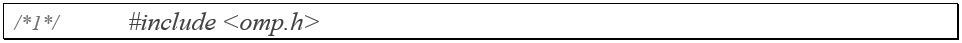
\includegraphics[width=1\linewidth]{includeOpenMP}
	\end{figure}
	\par\textbf{Отличительные особенности.} Среди прочих технологий распараллеливания OpenMP выделяется следующими важными и характеристиками:
	\begin{itemize}
		\itemИнкрементное распараллеливание.
		\itemОбратная совместимость.
		\itemВысокий уровень абстракций.
		\itemНизкий коэффициент трансформации.
		\itemПоддержка крупнейшими  IT-гигантами. 
		\itemАвтоматическое масштабирование.
	\end{itemize}
	\par\textit{Инкрементное распараллеливание.}  OpenMP позволяет распараллеливать существующую последовательную программу в виде  небольших итераций-правок, на каждой из которых будет достигаться всё больший коэффициент распараллеленности программы. Эта особенность является уникальной, т.к. большинство других технологий предполагают существенное изменение структуры распараллеливаемой программы уже на первом этапе процесса распараллеливания, при этом первая работоспособная параллельная версия программы появляется после длительного процесса отладки и программирования новых компонентов, которые неизбежно добавляются при распараллеливании. OpenMP лишён этого недостатка.
	\par\textit{Обратная совместимость.} Большинство программных технологий развиваются с обеспечением обратной совместимости (backward compatibility), когда более новая версия программы поддерживает работоспособность старых файлов. Термин \textit{"прямая совместимость"} (forward compatibility) имеет противоположный смысл: файлы, созданные в программе новой версии, остаются работоспособными при использовании старой версии программы. В случае OpenMP это проявляется в том, что распараллеленная программа будет корректно скомпилирована в однопоточном режиме даже на старом компиляторе, который не поддерживает OpenMP. Важно отметить, что прямая совместимость обеспечивается, если при распараллеливании не используются библиотечные функции OpenMP, а присутствуют только препроцессорные директивы. При наличии библиотечных функций для обеспечения обратной совместимости потребуется написать функции-заглушки в файле "omp.h" (лишь немногие компиляторы умеют генерировать эти заглушки при использовании специального ключа).
	\par\textit{Высокий уровень абстракций.} Одна единственная препроцессораня директива OpenMP после обработки компилятором приводит к существенной трансформации исходной программы с добавлением большого количества новой логики, отвечающей за определение доступного в системе количества процессоров, за запуск и уничтожение потоков, за распределение работы между потоками и т.п. Все эти операции OpenMP берёт на себя,  взамен программист получает набор очень высокоуровневых инструментов распараллеливания. У высокоуровневых языков есть и традиционная тёмная сторона: в OpenMP отсутствует возможность изменить некоторую внутренние детали работы с потоками (например, нельзя установить аффинность  потоков или уменьшить накладные расходы на создание/удаление потоков).
	\par\textit{Низкий коэффициент параллельной трансформации (КПТ).} При распараллеливании существующей последовательной программы приходится вносить в неё достаточно большое количество изменений. Пусть КПТ – это отношение строк нового программного кода, который добавился в результате распараллеливания, к общему количеству строк кода в программе. В OpenMP КПТ обычно существенно ниже, чем у большинства других технологий распараллеливания. Это объясняется высоким уровнем абстракции языка OpenMP (см. предыдущий пункт). 
	\par\textit{Поддержка крупнейшими  IT-гигантами.} Уже при разработке\\ OpenMP о его поддержке заявили крупнейшие игроки IT-мира. Это обеспечило не только высокое качество разработки стандарта, но и наличие готовых реализаций стандарта в популярных компиляторах. Несмотря на прошедшие два десятка лет OpenMP не растерял приверженцев и поддержка новейших версий OpenMP с достаточно малой задержкой появляется в компиляторах. Например, при текущей версии стандарта OpenMP 4.5 наиболее популярные компиляторы уже поддерживают версию OpenMP 4.0. Исключением является только фирма Microsoft. Их компилятор вот уже несколько версий неизменно поддерживает только \\OpenMP 2.0. 
	\par\textit{Автоматическое масштабирование.}  Низкоуровневые технологии распараллеливания (POSIX Threads, OpenCL) предлагают программисту вручную управлять количеством создаваемых потоков при выполнении параллельной работы. Это обеспечивает возможность гибко управлять и настраивать процесс создания потоков в зависимости от количества доступных системе процессоров (ядер), но при этом требует от программиста большой количества неавтоматизируемой работы. В OpenMP управление масштабированием происходит в автоматическом режиме, т.е. OpenMP сам запрашивает у операционной системы количество доступных процессоров и выбирает количество создаваемых потоков. Но при необходимости OpenMP оставляет возможность устанавливать требуемое количество потоков вручную.
	\par\textbf{Примеры OpenMP-программ.}
}
	{ %section3_4
	\subsection{Технология OpenMP}
	\label{OpenMP:section}
	\par\textbf{Краткая характеристика технологии.} Первая версия стандарта OpenMP появилась в 1997 году при поддержке крупнейших IT-компаний мира (Intel, IBM, AMD, HP, Nvidia и др.). Целью нового стандарта было предложить кроссплатформенный инструмент для распараллеливания, который был бы более высокоуровневый, чем API управления потоками, предлагаемые операционной системой. На данный момент OpenMP стандартизована для трёх языков программирования: С, С++ и Фортран.
	\par\textbf{Поддержка компиляторами.} Абсолютное большинство существующих современных компиляторов С/С++ поддерживают OpenMP версии 2.0 (например, как gcc, так и Visual Studio). Однако лишь немногие компиляторы поддерживают более новую версию OpenMP 4.0, поэтому далее при изложении материала будет в качестве ''общего знаменателя'' использоваться технология OpenMP 2.0.
	\par OpenMP определяет набор директив препроцессору, которые дают указание компилятору заменить следующий за ними исходный код на его параллельную версию с помощью доступных компилятору средств, например с помощью POSIX Threads в Linux или Windows Threads в операционных системах Microsoft. Для корректной трансляции директив необходимо при компиляции указать специальный ключ, значение которого зависит от компилятора (примеры приведены в таблице~\ref{compilerOpenMP:table}).
	\begin{table}[H]
		\caption{Ключи компиляторов для запуска OpenMP}
		\label{compilerOpenMP:table}
		\begin{center}
			\begin{tabular}{|c|c|}
				\hline
				\textbf{Название компилятора} & \specialcell{\textbf{Ключ компилятору для включения} \\  \textbf{OpenMP}} \\
				\hline
				Gcc & -fopenmp \\
				\hline
				icc (Intel C/C++ compiler) & -qopenmp \\
				\hline
				Sun C/C++ compiler & -xopenmp \\
				\hline
				Visual Studio C/C++ compiler & /openmp \\
				\hline
				PGI (Nvidia C/C++ compiler) & -mp \\
				\hline
			\end{tabular}
		\end{center}
	\end{table}
	\parПомимо препроцессорных директив, OpenMP определяет набор библиотечных функций, для вызова которых в исходном коде потребуется подключить заголовочный файл OpenMP:
	\begin{figure}[H]
		\lstinputlisting{includeOpenMP.cpp}
	\end{figure}
	\par\textbf{Отличительные особенности.} Среди прочих технологий распараллеливания OpenMP выделяется следующими важными и характеристиками:
	\begin{itemize}
		\itemИнкрементное распараллеливание.
		\itemОбратная совместимость.
		\itemВысокий уровень абстракций.
		\itemНизкий коэффициент трансформации.
		\itemПоддержка крупнейшими  IT-гигантами. 
		\itemАвтоматическое масштабирование.
	\end{itemize}
	\par\textit{Инкрементное распараллеливание.}  OpenMP позволяет распараллеливать существующую последовательную программу с помощью небольших итераций-правок, на каждой из которых будет достигаться всё больший коэффициент распараллеленности программы. Эта особенность является уникальной, т.к. большинство других технологий предполагают существенное изменение структуры распараллеливаемой программы уже на первом этапе процесса распараллеливания, т.е. первая работоспособная параллельная версия программы появляется после длительного процесса отладки и программирования новых компонентов, которые неизбежно добавляются при распараллеливании. OpenMP лишён этого недостатка.
	\par\textit{Обратная совместимость.} Большинство программных технологий развиваются с обеспечением обратной совместимости (backward \\compatibility), когда более новая версия программы поддерживает работоспособность старых файлов. Термин \textit{''прямая совместимость''} (forward compatibility) имеет противоположный смысл: файлы, созданные в программе новой версии, остаются работоспособными при использовании старой версии программы. В случае OpenMP это проявляется в том, что распараллеленная программа будет корректно скомпилирована в однопоточном режиме даже на старом компиляторе, который не поддерживает OpenMP. Важно отметить, что прямая совместимость обеспечивается, если при распараллеливании не используются библиотечные функции OpenMP, а присутствуют только препроцессорные директивы. При наличии библиотечных функций для обеспечения обратной совместимости потребуется написать функции-заглушки в файле ''omp.h'' (некоторые компиляторы умеют генерировать эти заглушки при использовании специального ключа).
	\par\textit{Высокий уровень абстракций.} Одна единственная препроцессорная директива OpenMP после обработки компилятором приводит к существенной трансформации исходной программы с добавлением большого количества новой логики, отвечающей за определение доступного в системе количества процессоров, за запуск и уничтожение потоков, за распределение работы между потоками и т.п. Все эти операции OpenMP берёт на себя, взамен программист получает набор очень высокоуровневых инструментов распараллеливания. У высокоуровневых языков есть и традиционный недостаток: в OpenMP отсутствует возможность изменить некоторые внутренние детали работы с потоками (например, нельзя установить аффинность потоков или уменьшить накладные расходы на создание/удаление потоков).
	\par\textit{Низкий коэффициент параллельной трансформации (КПТ).} При распараллеливании существующей последовательной программы приходится вносить в неё достаточно большое количество изменений. Пусть КПТ – это отношение строк нового программного кода, который добавился в результате распараллеливания, к общему количеству строк кода в программе. В OpenMP КПТ обычно существенно ниже, чем у большинства других технологий распараллеливания. Это объясняется высоким уровнем абстракции языка OpenMP (см. предыдущий пункт). 
	\par\textit{Поддержка крупнейшими  IT-гигантами.} Уже при разработке\\ OpenMP о его поддержке заявили крупнейшие игроки IT-мира. Это обеспечило не только высокое качество разработки стандарта, но и наличие готовых реализаций стандарта в популярных компиляторах. Несмотря на прошедшие два десятка лет OpenMP не растерял приверженцев и поддержка новейших версий OpenMP с достаточно малой задержкой появляется в компиляторах. Например, при текущей версии стандарта OpenMP 4.5 наиболее популярные компиляторы уже поддерживают версию OpenMP 4.0. Исключением является только фирма Microsoft. Их компилятор вот уже несколько версий неизменно поддерживает только \\OpenMP 2.0. 
	\par\textit{Автоматическое масштабирование.}  Низкоуровневые технологии распараллеливания (POSIX Threads, OpenCL) предлагают программисту вручную управлять количеством создаваемых потоков при выполнении параллельной работы. Это обеспечивает возможность гибко управлять и настраивать процесс создания потоков в зависимости от количества доступных системе процессоров (ядер), но при этом требует от программиста большое количество неавтоматизируемой работы. В OpenMP управление масштабированием происходит в автоматическом режиме, т.е. OpenMP сам запрашивает у операционной системы количество доступных процессоров и выбирает количество создаваемых потоков. Но при необходимости OpenMP оставляет возможность устанавливать требуемое количество потоков вручную.
	\par\textbf{Примеры OpenMP-программ.} Рассмотрим ниже простейшие примеры работающих параллельных программ, начиная с традиционного для программирования примера ''Hello, World'':
	\begin{figure}[H]
		\lstinputlisting{OpenMPExample1.cpp}
	\end{figure}
	\parРезультатом работы будет выведенное несколько раз в консоль сообщение. Количество сообщений определяется количеством логических процессоров, доступных системе (например, при использовании технологии HyperThreading при двух ядрах количество логических процессоров будет равно четырём). 
	\parДействие директивы pragma распространяется на следующий за ней исполняемый блок. В данном случае это вызов функции printf, но можно было бы заключить произвольное количество операций в фигурные скобки, чтобы расширить исполняемый блок:
	\begin{figure}[H]
		\lstinputlisting{OpenMPExample2.cpp}
	\end{figure}
	В этой программе заключенный в фигурные скобки блок операций выполняется одновременно на нескольких ядрах. При этом в строке 5 процессору даётся указание выполнить операцию ''i++'' атомарно, т.е. не параллельно, а последовательно каждым из потоков. 
	\parС одной стороны, это приводит к тому, что операция инкремента перестаёт быть распараллеленной, что снижает скорость многоядерного выполнения. С другой стороны, директива atomic в данном случае необходима, т.к. иначе могла бы возникнуть сложно обнаружимая проблема с гонкой данных, проявляющаяся в конфликте при записи данных в общую область памяти одновременно несколькими потоками в переменную i. Заметим, что директива atomic может применяться только для однострочных простых команд присваивания. 
	\parДля изоляции более сложных составных команд с возможным вызовом пользовательских и системных функций следует использовать директиву critical, которая допускает (в отличие от директивы atomic) возможность расширения своей области действия на блок операций, заключённый в фигурные скобки? при этом каждая critical-секция может иметь имя, позволяющее сгруппировать разные критические секции по этому имени, чтобы предотвратить появление единой распределённой по всей программе критической секции:
	\begin{figure}[H]
		\lstinputlisting{OpenMPExample3.cpp}
	\end{figure}
	\parВ этом случае функция printf в строке 4 выполняется всеми потоками параллельно, что может привести к перемешиванию выводимых символов. Напротив, функция printf в строке 8 выполняется потоками строго по очереди, что предотвращает возможные конфликты между ними, однако замедляет выполнение программы из-за искусственного ограничения коэффициента распараллеленности.
	\parПриведём пример распараллеливания программы, содержащей последовательный вызов функций run\textunderscore function1 и run\textunderscore function2, которые не зависят друг от друга (т.е. не используют общих данных и результаты работы одной не влияют на результаты работы другой) и поэтому допускающих удобное \textit{распараллеливание по инструкциям} в чистом виде:
	\begin{figure}[H]
		\lstinputlisting{OpenMPExample4.cpp}
	\end{figure}
	\parРассмотрим пример распараллеливания цикла с использованием OpenMP. Пусть в каждую ячейку одномерного массива нужно записать индекс этой ячейки, возведённый в шестую степень:
	\begin{figure}[H]
		\lstinputlisting{OpenMPExample5.cpp}
	\end{figure}
	\parПусть указанная программа выполняется на двухъядерном процессоре. Тогда первый процессор рассчитает значения с a[0] по a[4], второй процессор – значения с a[5] по a[9]. Видимо, что при записи в массив процессору не мешают друг другу, т.к. работают с разными частями массива. Попробуем оптимизировать предыдущий вариант, сократив количество операций умножения для возведения в шестую степень:
	\begin{figure}[H]
		\lstinputlisting{OpenMPExample6.cpp}
	\end{figure}
	\parВ указанном случае программа будет корректно работать только при наличии одного процессора (ядра). При наличии нескольких ядер будет наблюдаться состояние гонки данных при одновременной записи нового значения в переменную tmp (строка 4) несколькими потоками, в результате массив будет заполнен некорректно. Например, пусть первый поток, выполняющий итерацию i=2 записал в tmp число 8. Теперь при вычислении a[2] поток попытается записать число 8*8, однако если до начала строки 5 успеет вклиниться второй поток, работающей с итерацией i=7, то значение tmp превратиться в 7*7*7, а значение a[2], рассчитываемое первым потоком, превратиться в $7^6$, вместо положенных 64. Исправим допущенную ошибку следующим образом:
	\begin{figure}[H]
		\lstinputlisting{OpenMPExample7.cpp}
	\end{figure}
	\parВ директиве препроцессору появился новый элемент: private. Этот элемент задаёт через запятую перечень локальных (приватных) для каждого потока переменных. В данном случае такая переменная одна: tmp. Другой равноценный способ исправить ошибку – это перенести объявление переменной ''int tmp'' внутрь параллельной области, что заставить OpenMP считать эту переменную локальной для каждого потока. Может возникнуть вопрос, почему в перечень локальных переменных не добавлена i. Ответ не очевиден: OpenMP по умолчанию считает переменную распараллеливаемого цикла локальной.
	\parЛюбая переменная, объявленная внутри параллельной области, считается в OpenMP локальной, поэтому такие переменные не нужно указывать в списке. Любая переменная, объявленная вне этой области является глобальной (в нашем случае глобальной переменной является указатель на массив $а$). Но если требуется явным образом указать на глобальность переменной, следует рядом с командой private использовать команду shared(x,\ldots), где x задаёт список глобальных переменных.
	\parРассмотрим пример, в котором нужно рассчитать сумму и для дальнейшего исполнения формировать массив элементов следующего ряда: $\{\;1^i,\;2^i,\;3^i,\;4^i,\;5^i\;\}$ для различных значений $i$, например: $i\;=\;1,\;2,\;3$. Приведём ниже решение поставленной задачи, но умышленно допустим в ней ошибку:
	\begin{figure}[H]
		\lstinputlisting{OpenMPExample8.cpp}
	\end{figure}
	\parВ строке 2 происходит запуск параллельной области, но программист забывает указать, что переменные j и массив tmp должны быть локальными для каждого треда. Действительно, в строке 4 происходит инкремент общей для потоков переменной j, который выполняется всеми потоками одновременно. В этой ситуации потоки могут помешать друг другу, переписав чужое значение j. Исправим обе ошибки следующим образом:
	\begin{figure}[H]
		\lstinputlisting{OpenMPExample9.cpp}
	\end{figure}
	\parВидим, что теперь переменная j явным образом обозначена локальной (private). С массивом tmp решение другое – он весь помещается внутрь параллельной области (т.е. у каждого потока будет свой собственный не зависимый от других экземпляр массива tmp). Почему же нельзя было просто указать переменную tmp в перечне команды private, как это было сделано для j? Ответ связан со спецификой языка С: переменная tmp является указателем, который при работе цикла не меняется, но меняется содержимое памяти, на которое указывает tmp. Это значит, что указывание tmp в качестве private-переменной не решило бы проблему с гонками данных, т.к. все потоки получили бы один и тот же адрес tmp и мешали бы друг другу, записывая новые значения по этому адресу.
	\parРассмотрим ещё одну типичную для параллельного программирования ошибку. Следующая программа считает сумму чисел от 1 до 100:
	\begin{figure}[H]
		\lstinputlisting{OpenMPExample10.cpp}
	\end{figure}
	\parПеременная sum является глобальной, поэтому при попытке записать в неё новое значение потоки будут мешать друг другу. Чтобы исправить ошибку, нам придётся использовать локальную для каждого потока сумму, а затем потребуется сложить все эти локальные суммы:
	\begin{figure}[H]
		\lstinputlisting{OpenMPExample11.cpp}
	\end{figure}
	Видим начало параллельной области в строке 2 – именно в этом месте OpenMP создаёт несколько потоков. В строке 6 новые потоки не создаются (т.к. отсутствует ключевое слово parallel), но входящие в цикл потоке делят итерации между собой, а не выполняют каждый все итерации целиком. В строке 8 рассчитавший свою частичную сумму поток пытается прибавить эту сумму к общей сумме. Это приходится делать с помощью директивы atomic, которая гарантирует, что потоки не будут мешать друг другу при перезаписи sum. 
	\parЕщё один сложный момент – это повторная инициализация переменной sum\textunderscore private в строке 4: необходимость в этом возникает, т.к. OpenMP не инициализирует локальные переменные, даже если есть глобальные переменные с идентичными именами. Подобное решение призвано уменьшить накладные расходы на копирование переменных.
	\parОписанный подход является работоспособным, однако он почти не используется на практике, т.к. стандарт OpenMP для целого класса подобных задач предлагает более высокоуровневое и простое решение. Оно состоит в использовании команды reduction:
	\begin{figure}[H]
		\lstinputlisting{OpenMPExample12.cpp}
	\end{figure}
	\parКоманда reduction помечает перечисленный переменные как локальные, а в конце параллельной области все локальные переменные объединяет (агрегирует) в одну глобальную переменную с тем же именем, используя указанную операцию. В нашем случае операцией является суммирование. Но OpenMP допускает вместо знака ''+'' использовать ''*'', ''-'', ''/''. Важно, что reduction кроме прочего выполняет инициализацию переменных не значениями исходных глобальных переменных, а наиболее соответствующими логики агрегации значениями: например, при суммировании переменная инициализируется нулём, а при умножении – единицей.
	\parПри распараллеливании цикла может оказаться, что итерации неравноценны по количеству выполняемой работы между собой. Это может привести к тому, что один поток справится с выделенной частью итераций намного быстрее второго потока и будет простаивать. Для решения этой проблемы OpenMP предлагает четыре разных способа распределения итераций по потокам. 
	\begin{itemize}
		\item\textit{Способ по умолчанию:} при этом итерации делятся на количество частей, равное количеству потоков; каждый поток выполняет после этого свою часть и не может взять чужую работу.
		\item\textit{Статическое распределение (static):} итерации разбиваются на части указанного пользователям размера; затем ещё до начала работы каждый поток получает фиксированное количество частей и выполняет только их без возможности переключиться на другие.
		\item\textit{Динамическое распределение (dynamic):} итерации разбиваются на части указанного пользователям размера; затем сразу начинается работа цикла и каждый поток получает новую часть итераций по мере завершения работы над предыдущей.
		\item\textit{Управляемое распределение (guided):} компилятор разбивает итерации на количество частей, равное удвоенному количеству потоков; затем сразу начинается работа цикла и каждый поток получает новую часть итераций по мере завершения работы над предыдущей, при этом размер нововыданной части уменьшается по сравнению с предыдущим разом, но не может стать меньше указанного пользователем константного значения.
	\end{itemize}
	\parУпомянутый в каждом из методов пользовательский параметр называется chunk\textunderscore size. Каждый из указанных методов имеет свою область применения, в которой он может обеспечить максимальное параллельное ускорение. Отметим, что режимы dynamic и guided несмотря на свою логичность имеют и свои недостатки: они требуют существенных накладных расходов во время работы цикла по сравнению со static. Также важно понимать, что при выборе числа chunk\textunderscore size необходимо учитывать особенности работы механизма кеширования.
	\parРассмотрим пример статического распределения итераций:
	\begin{figure}[H]
		\lstinputlisting{OpenMPExample13.cpp}
	\end{figure}
	\parПри наличии трёх ядер OpenMP создаст три потока. Первому потоку достанутся итерации $i=1,\;4,\;7,\;…,\;97$ второму – итерации $i=2,\;5,\;8,\;…,\;98$, третьему – итерации $i=3,\;6,\;9,\;…,\;99$. Обратим внимание, что выбор малого значения параметра chunk\textunderscore size = 1 в данном случае не имеет каких-либо негативных эффектов. Однако если бы i использовалась в качестве индекса при обращении к массиву, то предложенный вариант разбиения привёл бы к обращению в память не подряд по последовательным адресам, а разреженно с шагом 3, что ухудшило бы показатели cache hit при использовании кэширования.
	\parРассмотрим ещё один пример: 
	\begin{figure}[H]
		\lstinputlisting{OpenMPExample14.cpp}
	\end{figure}
	\parЗдесь приводится пример, как можно указать OpenMP количество создаваемых потоков с помощью опции num\textunderscore threads (строка 2), не ориентируясь на реально доступное количество ядер (процессоров) на компьютере. Далее три созданных потока делят между собой 100 итераций уже знакомым нам способом. Однако опция nowait позволяет первому справившемуся с работой потоку не дожидаться остальных, а перейти к следующей за циклом работе. За циклом в параллельном режиме выполняются две функции (строки 9 и 11). Каждая из функций заключена в секцию (section), которые должны иметь родительский элемент sections. В итоге первый освободившийся после цикла поток займётся вычислением функции в строке 9. Второй освободившийся поток вычислит функцию в строке 11. Третьему потоку не достанется работы помимо своей доли итераций в первом цикле.
Общим требованием OpenMP к распараллеливаемым циклам является их \textit{каноничность}. Цикл for называется \textit{каноническим}, если можно при его начале заранее рассчитать количество предстоящих итераций. Это возможно, если одновременно выполняются следующие условия:
	\begin{itemize}
		\itemвнутри цикла нет операций break и return;
		\itemвнутри цикла нет операции goto, ведущей вовне цикла;
		\itemпеременная цикла (итератор) не изменяется внутри цикла;
	\end{itemize}
	При этом запись цикла должна иметь вид ''for (i = A; i < B; i+=C)'', где числа A, B, C не должны меняться во время работы цикла. Второй параметр цикла может использовать не только знак ''<'', но и  ''>'',  ''>='',  ''<=''. Третий параметр цикла может не только инкрементировать, но декрементировать переменную цикла (допускается краткая форма записи ''i++'').
	\parЕсли итерация k влияет на результаты итерации m, то цикл нельзя распараллеливать, т.к. нельзя заранее предсказать порядок завершения итераций несколькими потоками.  Ответственность за обнаружение таких конфликтов лежит на программисте. Например, OpenMP не обнаружит взаимозависимость итераций и скомпилирует следующую программу:
	\begin{figure}[H]
		\lstinputlisting{OpenMPExample15.cpp}
	\end{figure}
	\parВ этой программе поток 0 скорее всего не успеет заполнить элемент a[9] к тому моменту, когда поток 1 будет вычислять значение a[10] = 2*a[9].
	\par
}
}
	{ %section4
	\section{Лабораторная работа №1. «Автоматическое распараллеливание программ»}
	{ %section4_1
	\subsection{Порядок выполнения работы}
	\begin{enumerate}
		\itemНа компьютере с многоядерным процессором установить ОС Linux и компилятор GCC версии не ниже 4.7.2. При невозможности установить Linux или отсутствии компьютера с многоядерным процессором можно выполнять лабораторную работу на виртуальной машине.
		\itemНа языке Cи написать консольную программу lab1.c, решающую задачу, указанную в п.IV (см. ниже). В программе нельзя использовать библиотечные функции сортировки, выполнения матричных операций и расчёта статистических величин.  В программе
нельзя использовать библиотечные функции, отсутствующие в стандартных заголовочных файлах stdio.h, stdlib.h, math.h, sys/time.h. Задача должна решаться 50 раз с разными начальными значениями генератора случайных чисел (ГСЧ).  Структура программы примерно следующая:
			\begin{figure}[H]
				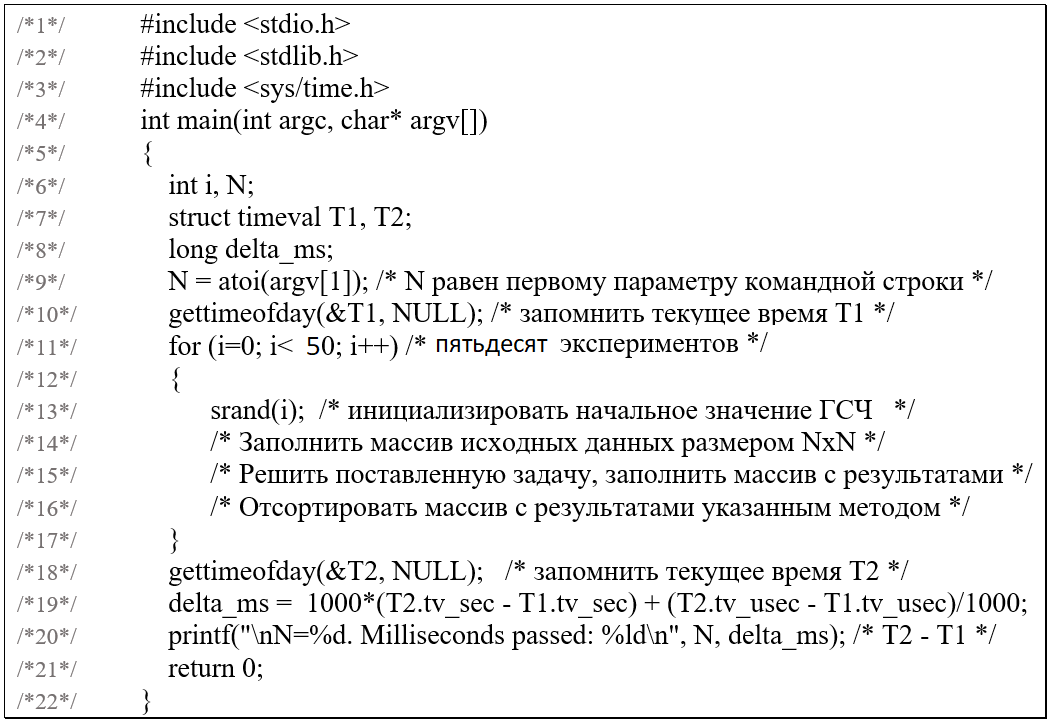
\includegraphics[width=1\linewidth]{lab1Example}
			\end{figure}
		\itemСкомпилировать написанную программу без использования автоматического распараллеливания с помощью следующей команды: /home/user/gcc -O2 -Wall -Werror -o lab1-seq lab1.c
		\itemСкомпилировать написанную программу, используя встроенное в gcc средство автоматического распараллеливания Graphite с помощью следующей команды “/home/user/gcc -O2 -Wall -Werror -floop-parallelize-all -ftree-parallelize-loops=K lab1.c -o lab1-par-K” (переменной K поочерёдно присвоить хотя бы 4 различных целых значений, выбор обосновать).
		\itemВ результате получится одна нераспараллеленная программа и десять распараллеленных.
		\itemЗакрыть все работающие в операционной системе прикладные программы (включая Winamp, uTorrent, браузеры и Skype), чтобы они не влияли на результаты последующих экспериментов.
		\itemЗапускать файл lab1-seq из командной строки, увеличивая значения N до значения N1, при котором время выполнения превысит 0.01 с. Подобным образом найти значение N=N2, при котором время выполнения превысит 2 с.
		\itemИспользуя найденные значения N1 и N2, выполнить следующие эксперименты (для автоматизации проведения экспериментов рекомендуется написать скрипт):
			\begin{itemize}
				\itemзапускать lab1-seq для значений \\$N\;=\;{N1,\;N1+\Delta,\;N1+2\Delta,\;N1+3\Delta,…,\;N2}$ и записывать получающиеся значения времени delta\textunderscore ms(N) в функцию $seq(N)$;
				\itemзапускать lab1-par-K для значений \\$N\;=\;{N1,\;N1+\Delta,\;N1+2\Delta,\;N1+3\Delta,…,\;N2}$ и записывать получающиеся значения времени delta\textunderscore ms(N) в функцию $par-K(N)$;
				\itemзначение $\Delta$ выбрать так: $\Delta\;=\;(N2\;-\;N1)/10$.
			\end{itemize}
		\itemНаписать отчёт о проделанной работе.
		\itemПодготовиться к устным вопросам на защите.
		\itemНайти вычислительную сложность алгоритма до и после распараллеливания, сравнить полученные результаты.
		\sloppy
		\item\textbf{Необязательное задание №1 (для получения оценки «четыре» и «пять»).} Провести аналогичные описанным эксперименты, используя вместо gcc компилятор Solaris Studio (или любой другой на своё усмотрение). При компиляции следует использовать следующие опции для автоматического распараллеливания: \\\verb+«solarisstudio -cc -O3 -xautopar -xloopinfo lab1.c»+
 		\item\textbf{Необязательное задание №2 (для получения оценки «пять»).} Это задание выполняется только после выполнения предыдущего пункта. Провести аналогичные описанным эксперименты, используя вместо gcc компилятор Intel ICC (или любой другой на своё усмотрение). В ICC следует при компиляции использовать следующие опции для автоматического распараллеливания: \verb+«icc -parallel -par-report -par-threshold K -o lab1-icc-par-K lab1.c»+.
	\end{enumerate}
	
}
	{ %section4_2
	\subsection{Состав отчета}
	\Large
	\begin{enumerate}
		\itemТитульный лист с названием вуза, ФИО студента и названием работы.
		\itemСодержание отчета (с указанием номера страниц и т.п.).
		\itemОписание решаемой задачи (взять из п.I и п.IV).
		\itemКраткая характеристика использованного для проведения экспериментов процессора, операционной системы и компилятора GCC (официальное название, номер версии/модели, разрядность, количество ядер, ёмкость ОЗУ и т.п.).
		\itemПолный текст программы lab1.c в виде отдельного файла.
		\itemТаблицы значений и графики функций seq(N), par-K(N) с указанием величины параллельного ускорения.
		\itemПодробные выводы с анализом приведённых графиков и полученных результатов.
		\itemОтчёт предоставляется на бумажном носителе или на флешке.
	\end{enumerate}
}
	{ %section4_3
	\subsection{Подготовка к защите}
	\begin{enumerate}
		\itemУметь объяснить каждую строку программы, представленной в отчёте.
		\itemЗнать о назначении и основных особенностях GCC, а также о назначении всех использованных в работе ключей компиляции GCC.
		\itemЗнать материал лекции №1.
		\itemВзять с собой все нужные файлы для демонстрации работы программы.
	\end{enumerate}
}
	{ %section4_4
	\subsection{Варианты заданий}
	\Large\parВариант задания выбирается в соответствии с Таблицей. Порядок вычислений должен быть следующим:
	\begin{enumerate}
		\itemСформировать матрицу М1 размерностью N x N, заполнив её случайными вещественными числами, имеющими равномерный закон распределения в диапазоне от А до В (включительно).
		\itemИз получившейся матрицы М1 нужно сформировать матрицу М2 (размерностью N x N) в соответствии с параметром С вашего варианта. 
		\itemСформировать матрицу М3 (размерностью N x N), выполнив матричное умножение М3 = М1 х М2. 
		\itemСформировать вектор V размерностью N х 1, используя задание, указанное параметром D. 
		\itemПолученный вектор V необходимо отсортировать методом, указанным в параметре Е (для этого нельзя использовать библиотечные функции).
	\end{enumerate}
	\parПример таблицы с параметрами задания для одного студента:
	\begin{center}
		\begin{tabular}{|c|c|c|c|c|c|}
		\hline
		\textbf{ФИО студента} & \textbf{A} & \textbf{B} & \textbf{C} & \textbf{D} & \textbf{E} \\
		\hline
		Иванов Иван Иванович  & -5         & 8          & 3          & 1          & 11         \\
		\hline
		\end{tabular}
	\end{center}
	\parЗначения параметров ''А'' и ''В'' задают численное значение левой и правой границы случайных величин, генерируемых в ходе выполнения лабораторной работы. 	Параметр ''С'', определяющий метод получения матрицы М2, принимает значения от одного до семи, означающие:
	\begin{enumerate}
		\itemУмножение М1 на скаляр 5.
		\itemВычитание из матрицы М1 матрицы Е размером N x N.
		\itemТранспонирование матрицы М1.
		\itemИнвертирование знака матрицы М1.
		\itemКаждый элемент М2 равен синусу симметричного элемента в М1.
		\itemКаждый элемент М2 равен десятичному логарифму модуля симметричного элемента в М1.
		\itemКаждый элемент М2 равен элементу M1, умноженному на Х, где:
			\begin{itemize}
				\item X равен числу $\pi$(3,14159265358...), если сумма номера строки и номера столбца нечётная.
				\item X равен числу $e$(2,718281828...), если сумма номера строки и номера столбца чётная.
			\end{itemize}
	\end{enumerate}
	\parПараметр ''D'', определяющий способ формирования вектора V с результатами, принимает значения от одного до девяти, означающие:
	\begin{enumerate}
		\itemМатематическое ожидание каждой строки.
		\itemВыборочная дисперсия каждой строки.
		\itemКоэффициент вариации положительных элементов каждой строки.
		\itemВыборочное среднеквадратичное отклонение каждой строки.
		\itemМинимальный элемент каждой строки.
		\itemМаксимальный элемент каждой строки.
		\itemВыборочная дисперсия отрицательных элементов каждой строки.
		\itemМаксимальный среди отрицательных элементов каждой строки.
		\itemМатематическое ожидание отрицательных элементов.
	\end{enumerate}
	\parПараметр ''E'', определяющий метод сортировки вектора с результатами, принимает значения от одного до девяти, означающие:
	\begin{enumerate}
		\itemСортировка выбором (Selection sort).
		\itemСортировка Шелла (Shell sort) .
		\itemСортировка расчёской (Comb sort).
		\itemПирамидальная сортировка (сортировка кучи, Heapsort).
		\itemБыстрая сортировка (Quicksort).
		\itemПоразрядная сортировка (цифровая сортировка).
		\itemСортировка подсчётом (Counting sort).
		\itemГномья сортировка.
	\end{enumerate}
}
}

	{ %section5
	\section{Лабораторная работа №2. «Распараллеливание циклов в OpenMP»}
	{ %section5_1
	\subsection{Порядок выполнения работы}
	\begin{enumerate}
		\itemДобавить во все for-циклы в программе из ЛР №1 следующую директиву OpenMP: \\	
"\#pragma omp parallel for default(none) private(...) shared(...)". Наличие всех перечисленных параметров в указанной директиве является обязательным.
		\itemПроверить все for-циклы на внутренние зависимости по данным между итерациями. Если зависимости обнаружились, использовать для защиты критических секций директиву "\#pragma omp critical" или "\#pragma omp atomic" (если операция атомарна), или параметр reduction (предпочтительнее).
		\itemУбедиться, что получившаяся программа обладает свойством прямой совместимости с компиляторами, не поддерживающими OpenMP (для проверки этого можно скомпилировать программу без опции –fopenmp, в результате не должно быть сообщений об ошибках, а программа должна корректно работать).
		\itemПровести эксперименты, замеряя параллельное ускорения. По результатам экспериментов оставить только те директивы \#pragma omp for, которые дают прирост в параллельном ускорении. Привести сравнение графиков параллельного ускорения с ЛР№1, используя те же значения параметров N1 и N2, что и в ЛР№1. 
		\itemПровести эксперименты повторно (т.е. изначально не удаляя директивы \#pragma omp for), но добавив параметр "schedule" и варьируя в экспериментах тип расписания. Исследование нужно провести для всех возможных расписаний: static, dynamic, guided. Способ варьирования параметра chunk\textunderscore size выбрать самостоятельно (но должно быть не менее 5 точек варьирования).
		\itemПо результатам экспериментов оставить только те директивы, которые дают прирост в параллельном ускорении. Привести сравнение графиков параллельного ускорения с ЛР№1 и п.4. 
		\itemВыбрать из рассмотренных в п.4 и п.5 наилучший вариант и сформулировать условия, при которых наилучшие результаты получились бы при использовании других типов расписания.
		\itemНаписать отчёт о проделанной работе.
		\itemПодготовиться к устным вопросам на защите.
	\end{enumerate}
}
	{ %section5_2
	\subsection{Состав отчета}
	\begin{enumerate}
		\itemТитульный лист с названием вуза, ФИО студентов и названием работы.
		\itemСодержание отчета (с указанием номера страниц и т.п.).
		\itemКраткая характеристика использованного для проведения экспериментов процессора, операционной системы и компилятора (официальное название, номер версии/модели, разрядность, количество ядер, ёмкость ОЗУ, размер кэша и т.п.).
		\itemОписание особенностей конфигурации использованной параллельной библиотеки, включая описание последовательности шагов, предпринятых для установки библиотеки, и использованных опций компиляции.
		\itemПолный текст полученной параллельной программы, а также текст всех скриптов, использованных для компилирования программы и проведения экспериментов.
		\itemГрафики функций времени выполнения использованных программ, а также графики параллельного ускорения и параллельной эффективности для разных $N$ и $M$ (допускается совмещать несколько графиков в одной системе координат).
		\itemПодробные выводы с анализом приведённых графиков и полученных результатов. Отчёт предоставляется на бумажном носителе или на флешке.
	\end{enumerate}
}
	{ %section5_3
	\subsection{Подготовка к защите}
	\begin{enumerate}
		\itemУметь объяснить каждую строку программы, представленной в отчёте.
		\itemЗнать о назначении всех использованных в работе ключей компиляции.
		\itemЗнать материал лекции №2.
		\itemВзять с собой все нужные файлы для демонстрации работы программы.
	\end{enumerate}
}
}

	{ %section6
	\section{Лабораторная работа №3. «Распараллеливание циклов с помощью технологии OpenMP»}
	{ %section6_1
	\subsection{Порядок выполнения работы}
	\begin{enumerate}
		\itemЗаменить функцию rand на rand\textunderscore r и объяснить в отчёте, чем эти функции различаются, а также привести условия, при которых использование rand вместо rand\textunderscore r приведёт к ошибочным результатам работы. 
		\itemИспользуя функцию omp\textunderscore get\textunderscore wtime, измерить время выполнения каждого из пяти этапов программы (заполнение массива, умножение матриц и т.п.). Замер времени необходимо осуществить двумя методами:	
			\begin{itemize}
				\itemметод А – как среднее по 100 прогонам (использовать srand(i));
				\itemметод Б – как минимальное по 100 прогонам (использовать srand(константа)).	
			\end{itemize}
		\itemВывод в консоль (или в файл) информации о замеренном времени выполнения этапов нужно вынести за пределы основного цикла for (чтобы при распараллеливании треды не выполняли операции ввода/вывода).
		\itemИспользуя изученные на лекциях директивы OpenMP (parallel, parallel for, for, schedule, sections, barrier, critical и любые другие), написать параллельную версию программы, распараллелив каждый из пяти этапов вычислений. При этом этап сортировки распараллелить так: разбить массив на 2 равные части, отсортировать каждую из частей внутри OpenMP-секции (omp parallel sections), а затем объединить отсортированные части в одну.
		\itemЗадание на «пятёрку»: на этапе сортировки разбить массив не на 2 части, а на n частей, где n становится известным на этапе выполнения программы: n = omp\textunderscore get\textunderscore num\textunderscore procs()). 
		\itemПредусмотреть отладочный вывод на экран промежуточных результатов выполнения вычислений (это нужно для проверки во время защиты), но эксперименты проводить без отладочного вывода. 
		\itemЗадание на «пятёрку»: обеспечить прямую совместимость (forward compatibility) написанной параллельной программы. Для этого все вызываемые функции вида omp\textunderscore * нужно условно определить в препроцессорных директивах, например так: 	   
			\begin{figure}[H]
				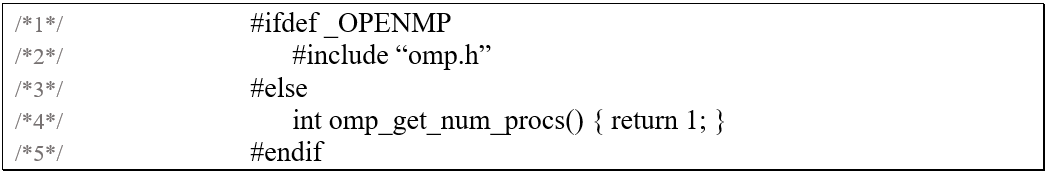
\includegraphics[width=1\textwidth]{lab3Example}
			\end{figure}
		\itemДоказательством того, что программа обладает прямой совместимостью, будет её успешная компиляция без ключа ''–fopenmp'' и корректность расчётов.
		\itemПровести эксперименты, замеряя параллельное ускорения на каждом из пяти этапов, самостоятельно выбрав диапазон значений N и количество экспериментов. Привести графики параллельного ускорения, рассчитанного методом А и методом Б, для каждого этапа и всей программы в целом. 
		\itemНаписать отчёт о проделанной работе с подробными выводами и комментариями полученных результатов (сравнить метод А и метод Б; объяснить влияние параллельного ускорения отдельных этапов на параллельное ускорение всей программы).
	\end{enumerate}
}
	{ %section6_2
	\subsection{Состав отчета}
	\begin{enumerate}
		\itemТитульный лист с названием вуза, ФИО студентов и названием работы.
		\itemСодержание отчета (с указанием номера страниц и т.п.).
		\itemКраткое описание решаемой задачи.
		\itemХарактеристика использованного для проведения экспериментов процессора, операционной системы и компилятора GCC (точное название, номер версии/модели, разрядность, размер кэша, количество ядер и т.п.).
		\itemПолный текст программы с использованием параметра schedule.
		\itemПодробные выводы с анализом каждого из приведённых графиков.
		\itemОтчёт предоставляется в бумажном или электронном виде вместе с полным текстом программы. По требованию преподавателя нужно быть готовыми скомпилировать и запустить этот файл на компьютере в учебной аудитории (или своём ноутбуке).
	\end{enumerate}
}
	{ %section6_3
	\subsection{Подготовка к защите}
	\begin{enumerate}
		\itemУметь объяснить каждую строку программы, представленной в отчёте. Уметь объяснить выводы, полученные в результате работы.
		\itemЗнать назначение каждой директивы OpenMP, использованной в программе.
		\itemПо возможности прочитать материал об использованных директивах OpenMP в книге Антонова «Введение в OpenMP».
	\end{enumerate}
}
}

	{ %section7
	\section{Лабораторная работа №4. «Метод доверительных интервалов при измерении времени выполнения
параллельной OpenMP-программы»}
	{ %section7_1
	\subsection{Порядок выполнения работы}
	\begin{enumerate}
		\itemВ программе, полученной в результате выполнения ЛР-3, так изменить этап Generate, чтобы генерируемый набор случайных чисел не зависел от количества потоков, выполняющих программу. Например, на каждой итерации $i$ перед вызовом rand\textunderscore r можно вызывать функцию srand(f(i)), где f – произвольно выбранная функция. Можно придумать и использовать любой другой способ.
		\itemЗаменить вызовы функции gettimeofday на omp\textunderscore get\textunderscore wtime.
		\itemРаспараллелить вычисления на этапе Sort, для чего выполнить сортировку в два этапа: 
			\begin{itemize}
				\itemОтсортировать первую и вторую половину массива в двух независимых нитях (можно использовать OpenMP-директиву ''parallel sections''); 
				\itemОбъединить отсортированные половины в единый массив.
			\end{itemize}
		\itemНаписать функцию, которая один раз в секунду выводит в консоль сообщение о текущем проценте завершения работы программы. Указанную функцию необходимо запустить в отдельном потоке, параллельно работающем с основным вычислительным циклом.
		\itemОбеспечить прямую совместимость (forward compatibility) написанной параллельной программы. Для этого все вызываемые функции вида «omp\textunderscore *» можно условно переопределить в препроцессорных директивах, например, так:
			\begin{figure}[H]
				\lstinputlisting{lab4Example.cpp}
			\end{figure}
		\itemПровести эксперименты, варьируя $N$ от $min(\frac{N_x}{2},\;N_1)$ до $N_2$, где значения $N_1$ и $N_2$ взять из ЛР-1, а $N_x$ – это такое значение $N$, при котором накладные расходы на распараллеливание превышают выигрыш от распараллеливания. Написать отчёт о проделанной работе. Подготовиться к устным вопросам на защите.
		\item\textbf{Необязательное задание на «четвёрку» и «пятёрку».} Уменьшить количество итераций основного цикла с 100 до 10 и провести эксперименты, замеряя время выполнения следующими методами: 
			\begin{itemize}
				\itemИспользование минимального из десяти полученных замеров; 
				\itemРасчёт по десяти измерениям доверительного интервала с уровнем доверия 95\%.
			\end{itemize}
			Привести графики параллельного ускорения для обоих методов в одной системе координат, при этом нижнюю и верхнюю границу доверительного интервала следует привести двумя независимыми графиками.
		\item\textbf{Необязательное задание на «пятёрку»:} в п.3 задания на этапе Sort выполнить параллельную сортировку не двух частей массива, а $k$ частей в $k$ нитях (тредах), где $k$ – это количество процессоров (ядер) в системе, которое становится известным только на этапе выполнения программы с помощью команды \\«k = omp\textunderscore get\textunderscore num\textunderscore procs()».
	\end{enumerate}
}
	{ %section7_2
	\subsection{Состав отчета}
	\begin{enumerate}
		\itemТитульный лист с названием вуза, ФИО студентов и названием работы.
		\itemСодержание отчета (с указанием номера страниц и т.п.).
		\itemКраткое описание решаемой задачи.
		\itemХарактеристика использованного для проведения экспериментов  процессора, операционной системы и компилятора GCC  (точное название, номер версии/модели, разрядность, количество ядер и т.п.).
		\itemПолный текст распараллеленной программы.
		\itemПодробные выводы с анализом каждого из приведённых графиков.
	\end{enumerate}
	\parОтчёт предоставляется в бумажном или электронном виде вместе с полным текстом программы. По требованию преподавателя нужно быть готовыми скомпилировать и запустить этот файл на компьютере в учебной аудитории (или своём ноутбуке).
	\par
}
	{ %section7_3
	\subsection{Подготовка к защите}
	\Large
	\begin{enumerate}
		\itemУметь объяснить каждую строку программы, представленной в отчёте. Уметь объяснить выводы, полученные в результате работы.
		\itemЗнать назначение каждой директивы OpenMP, использованной в программе.
	\end{enumerate}
}
}

	{ %section8
	\section{Лабораторная работа №5. «Параллельное программирование с использованием стандарта POSIX Threads»}
	{ %section8_1
	\subsection{Порядок выполнения работы}
	\begin{enumerate}
		\itemВзять в качестве исходной OpenMP-программу из ЛР-4, в которой распараллелены все этапы вычисления. Убедиться, что в этой программе корректно реализован одновременный доступ к общей переменной, используемой для вывода в консоль процента завершения программы.
		\itemИзменить исходную программу так, чтобы вместо OpenMP-директив применялся стандарт «POSIX Threads»:
			\begin{itemize}
				\itemдля получения оценки \textbf{«3»} достаточно изменить только один этап (Generate, Map, Merge, Sort), который является узким местом (bottle neck), а также функцию вывода в консоль процента завершения программы;
				\itemдля получения оценки \textbf{«4»} и \textbf{«5»} необходимо изменить всю программу, но допускается в качестве расписания циклов использовать «schedule static»;
				\itemдля получения оценки \textbf{«5»} необходимо хотя бы один цикл распараллелить, реализовав вручную расписание «schedule dynamic» или «schedule guided».
			\end{itemize}
		\itemПровести эксперименты и по результатам выполнить сравнение работы двух параллельных программ («OpenMP» и «POSIX Threads»), которое должно описывать следующие аспекты работы обеих программ (для различных $N$):
			\begin{itemize}
				\itemполное время решения задачи;
				\itemпараллельное ускорение;
				\itemдоля времени, проводимого на каждом этапе вычисления («нормированная
диаграмма с областями и накоплением»);
				\itemколичество строк кода, добавленных при распараллеливании, а также грубая оценка
времени, потраченного на распараллеливание (накладные расходы программиста);
				\itemостальные аспекты, которые вы выяснили самостоятельно (\textbf{Обязательный пункт});
			\end{itemize}
	\end{enumerate}
}

	{ %section8_2
	\subsection{Состав отчета}
	\begin{enumerate}
		\itemТитульный лист с названием вуза, ФИО студентов и названием работы. Содержание отчета (с указанием номера страниц и т.п.).
		\itemКраткое описание решаемой задачи.
		\itemХарактеристика использованного для проведения экспериментов  процессора, операционной системы и компилятора GCC  (точное название, номер версии/модели, разрядность, количество ядер и т.п.).
		\itemПолный текст распараллеленной программы (для п.2 и п.3).
		\itemПодробные выводы с анализом каждого из приведённых графиков.
	\end{enumerate}
	\parОтчёт предоставляется в бумажном или электронном виде вместе с полным текстом программы. По требованию преподавателя нужно быть готовыми скомпилировать и запустить этот файл на компьютере в учебной аудитории (или своём ноутбуке).
	\par
}
	{ %section8_3
	\subsection{Подготовка к защите}
	\begin{enumerate}
		\itemУметь объяснить каждую строку программы, представленной в отчёте. 
		\itemУметь объяснить выводы, полученные в результате работы.
		\itemПодготовиться к ответам на вопросы по материалам лекции №5.
	\end{enumerate}
}
}

	{ %section9
	\section{Лабораторная работа №6. «Изучение технологии OpenCL»}
	{ %section9_1
	\subsection{Порядок выполнения работы}
	\begin{enumerate}
		\itemВам необходимо реализовать один (для оценки 3) или два (для оценки 4) этапа вашей программы из предыдущих лабораторных работ. При этом вычисления можно проводить как на CPU, так и на GPU (на своё усмотрение, но GPU предпочтительнее).
		\item\textbf{Дополнительной задание (оценка 5).}
			\begin{itemize}
				\itemВыполнение заданий для оценки 3 и 4.
				\itemРасчёт доверительного интервала. 
				\itemПосчитать время 2 способами: с помощью profiling и с помощью обычного замера (как в предыдущих заданиях).
				\itemОценить накладные расходы.
				\item* Необязательное задание для магистрантов с большим количеством свободного времени: Проводить вычисления совместно на GPU и CPU (т.е. итерации в некоторой обоснованной пропорции делятся между GPU и CPU, и параллельно на них выполняются).
			\end{itemize}
		\itemПри желании данную лабораторную работу можно написать на CUDA.
	\end{enumerate}
}
	{ %section9_2
	\subsection{Состав отчета}
	\Large
	\begin{enumerate}
		\itemТитульный лист с названием вуза, ФИО студентов и названием работы. Содержание отчета (с указанием номера страниц и т.п.).
		\itemКраткое описание решаемой задачи.
		\itemХарактеристика использованного для проведения экспериментов  процессора, операционной системы и компилятора GCC  (точное название, номер версии/модели, разрядность, количество ядер и т.п.).
		\itemПолный текст распараллеленной программы (для п.2 и п.3).
		\itemПодробные выводы.
	\end{enumerate}
	\parОтчёт предоставляется в бумажном или электронном виде вместе с полным текстом программы. По требованию преподавателя нужно быть готовыми скомпилировать и запустить этот файл на компьютере в учебной аудитории (или своём ноутбуке).
	\par
}
	{ %section8_3
	\subsection{Подготовка к защите}
	\begin{enumerate}
		\itemУметь объяснить каждую строку программы, представленной в отчёте. Уметь объяснить выводы, полученные в результате работы.
		\itemПрочитать раздел методички~\ref{OpenCL:section} \textit{Технология OpenCL}.
		\itemИзучить материал лекции по технологии OpenCL.
	\end{enumerate}
}
}

	{ %bibliography
	\phantomsection
	\section*{Список используемой литературы}
	\addcontentsline{toc}{section}{Список используемой литературы}
	\begin{enumerate}
		\sloppy
		\itemСоснин В.В., Балакшин П.В. Введение в параллельные вычисления. – СПб: Университет ИТМО, 2016. – 51 с.
		\item Top 500 supercomputers list. URL: \url{https://www.top500.org/} (дата обращения: 12.02.19).
		\itemВикипедия. Симметричная мультипроцессорность. URL: \url{https://ru.wikipedia.org/wiki/%D0%A1%D0%B8%D0%BC%D0%BC%D0%B5%D1%82%D1%80%D0%B8%D1%87%D0%BD%D0%B0%D1%8F_%D0%BC%D1%83%D0%BB%D1%8C%D1%82%D0%B8%D0%BF%D1%80%D0%BE%D1%86%D0%B5%D1%81%D1%81%D0%BE%D1%80%D0%BD%D0%BE%D1%81%D1%82%D1%8C} (дата обращения: 12.02.19).
		\itemВикипедия. Массово-параллельная архитектура. URL: \url{https://ru.wikipedia.org/wiki/%D0%9C%D0%B0%D1%81%D1%81%D0%BE%D0%B2%D0%BE-%D0%BF%D0%B0%D1%80%D0%B0%D0%BB%D0%BB%D0%B5%D0%BB%D1%8C%D0%BD%D0%B0%D1%8F_%D0%B0%D1%80%D1%85%D0%B8%D1%82%D0%B5%D0%BA%D1%82%D1%83%D1%80%D0%B0} (дата обращения: 12.02.19).
		\itemВикипедия. OpenCL. URL: \url{https://ru.wikipedia.org/wiki/OpenCL} (дата обращения: 13.02.19).
		\itemВведение в GPU-вычисления - CUDA/OpenCL. URL: \url{http://my-it-notes.com/2013/06/gpu-processing-intro-cuda-opencl/} (дата обращения: 13.02.19).
		\itemБастраков С.И. Программирование на OpenCL. - Нижний новгород: ННГУ, 2011.
		\item OpenCL – официальный сайт URL \url{:http://www.khronos.org/opencl/} (дата обращения: 13.02.19).
		\itemАнтонов А.С. Параллельное программирование с использованием технологии MPI. - Москва: МГУ, 2004. - 72 с.
		\itemАнтонов А.С. Параллельное программирование с использованием технологии OpenMP. - Москва: МГУ, 2009.- 78 с.
		\itemВикипедия. Параллельные вычисления. URL: \url{https://ru.wikipedia.org/wiki/%D0%9F%D0%B0%D1%80%D0%B0%D0%BB%D0%BB%D0%B5%D0%BB%D1%8C%D0%BD%D1%8B%D0%B5_%D0%B2%D1%8B%D1%87%D0%B8%D1%81%D0%BB%D0%B5%D0%BD%D0%B8%D1%8F}
		\itemВикипедия. Распределенный вычисления. URL: \url{https://ru.wikipedia.org/wiki/%D0%A0%D0%B0%D1%81%D0%BF%D1%80%D0%B5%D0%B4%D0%B5%D0%BB%D1%91%D0%BD%D0%BD%D1%8B%D0%B5_%D0%B2%D1%8B%D1%87%D0%B8%D1%81%D0%BB%D0%B5%D0%BD%D0%B8%D1%8F}

	\end{enumerate}
}
\end{document}